\chapter{Results} \label{results}
In this chapter, the detection and tracking performance of the model will be assessed. The first section will assess the detection model using evaluation metrics with some sample images of correct detections and failures. After, the tracker's performance in tracking sperms will be assessed, including those with occlusions and blurs.

\newpage
\section{Detection Result}
The model was trained for 70 epochs with the dataset and the hyperparameters already set up in the previous chapter. Figure \ref{final} shows the loss progression of the model during training.

\begin{figure}[h]
  \begin{minipage}{\linewidth}
  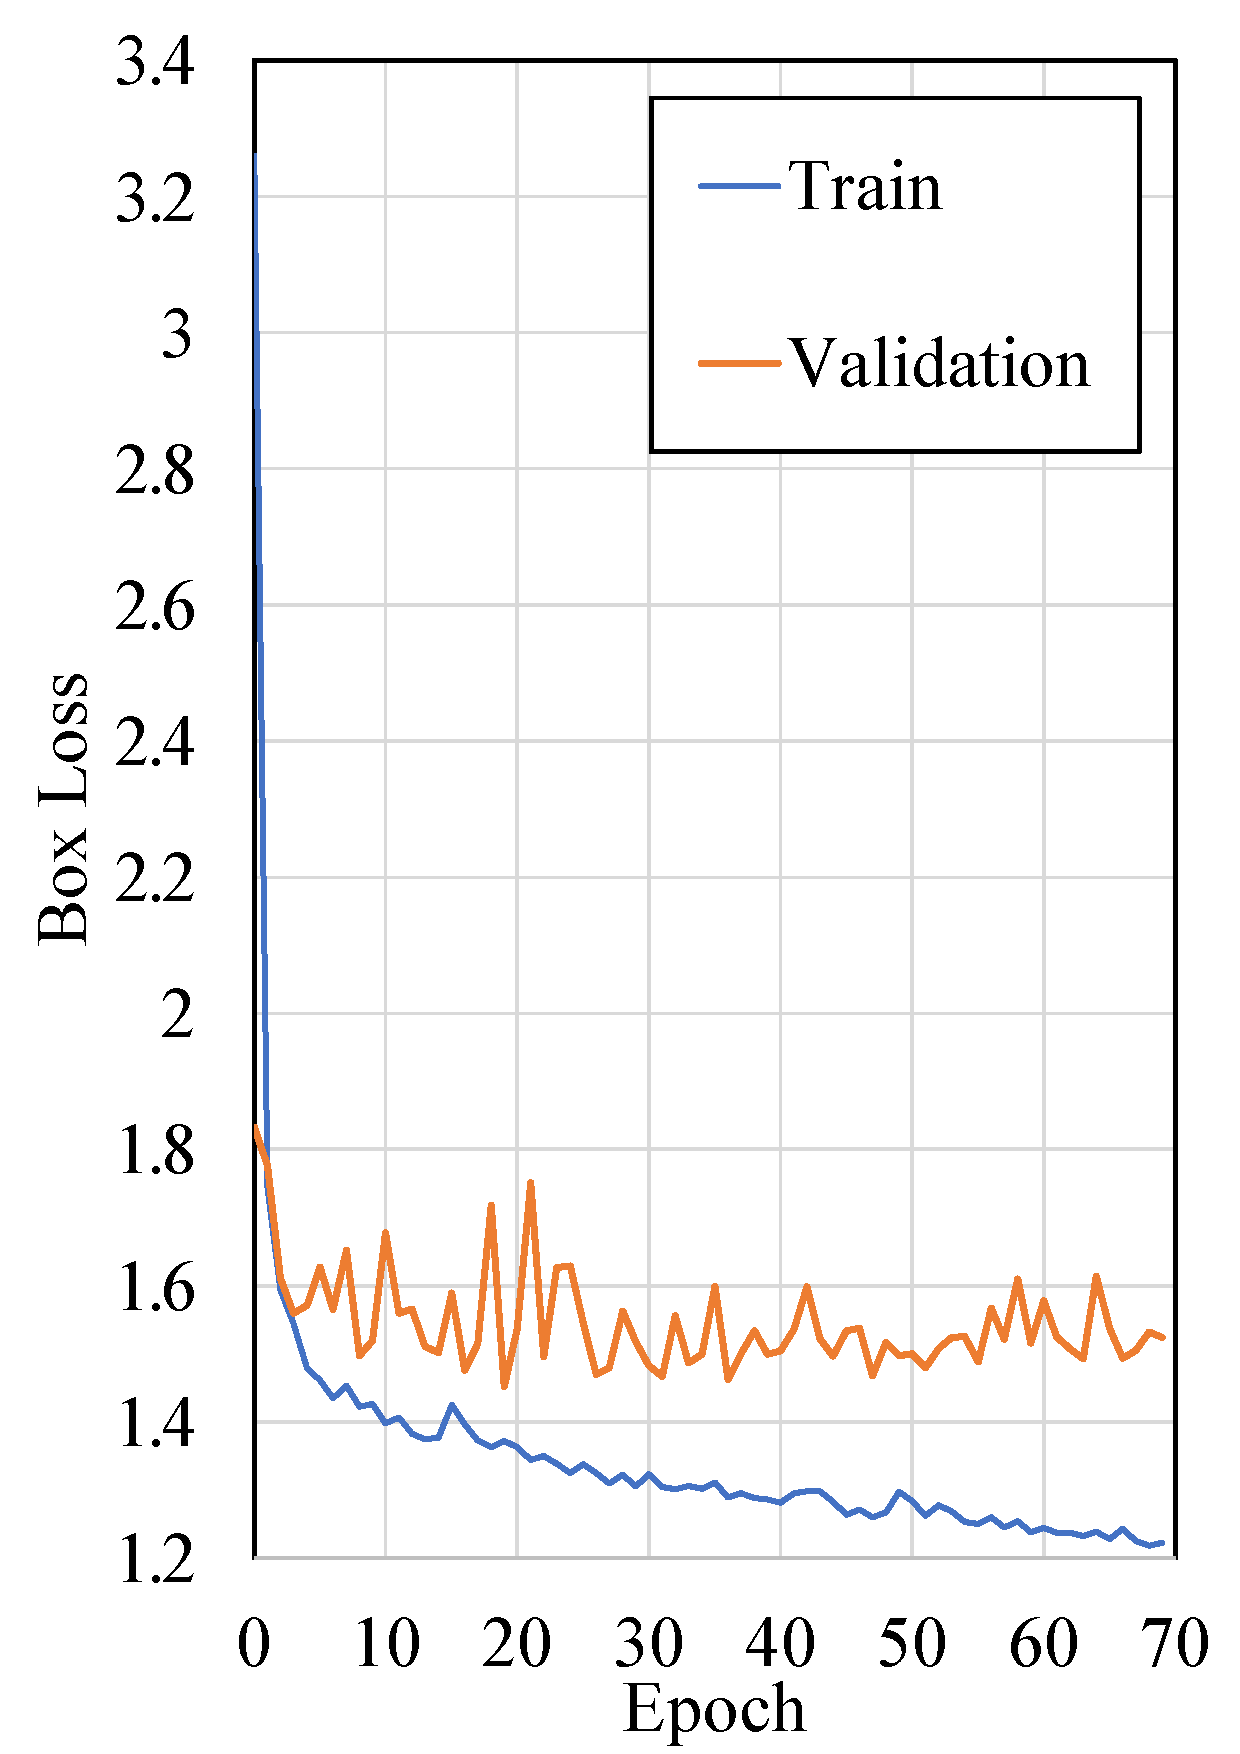
\includegraphics[width=0.333\linewidth]{Images/box2.pdf}\hfill
  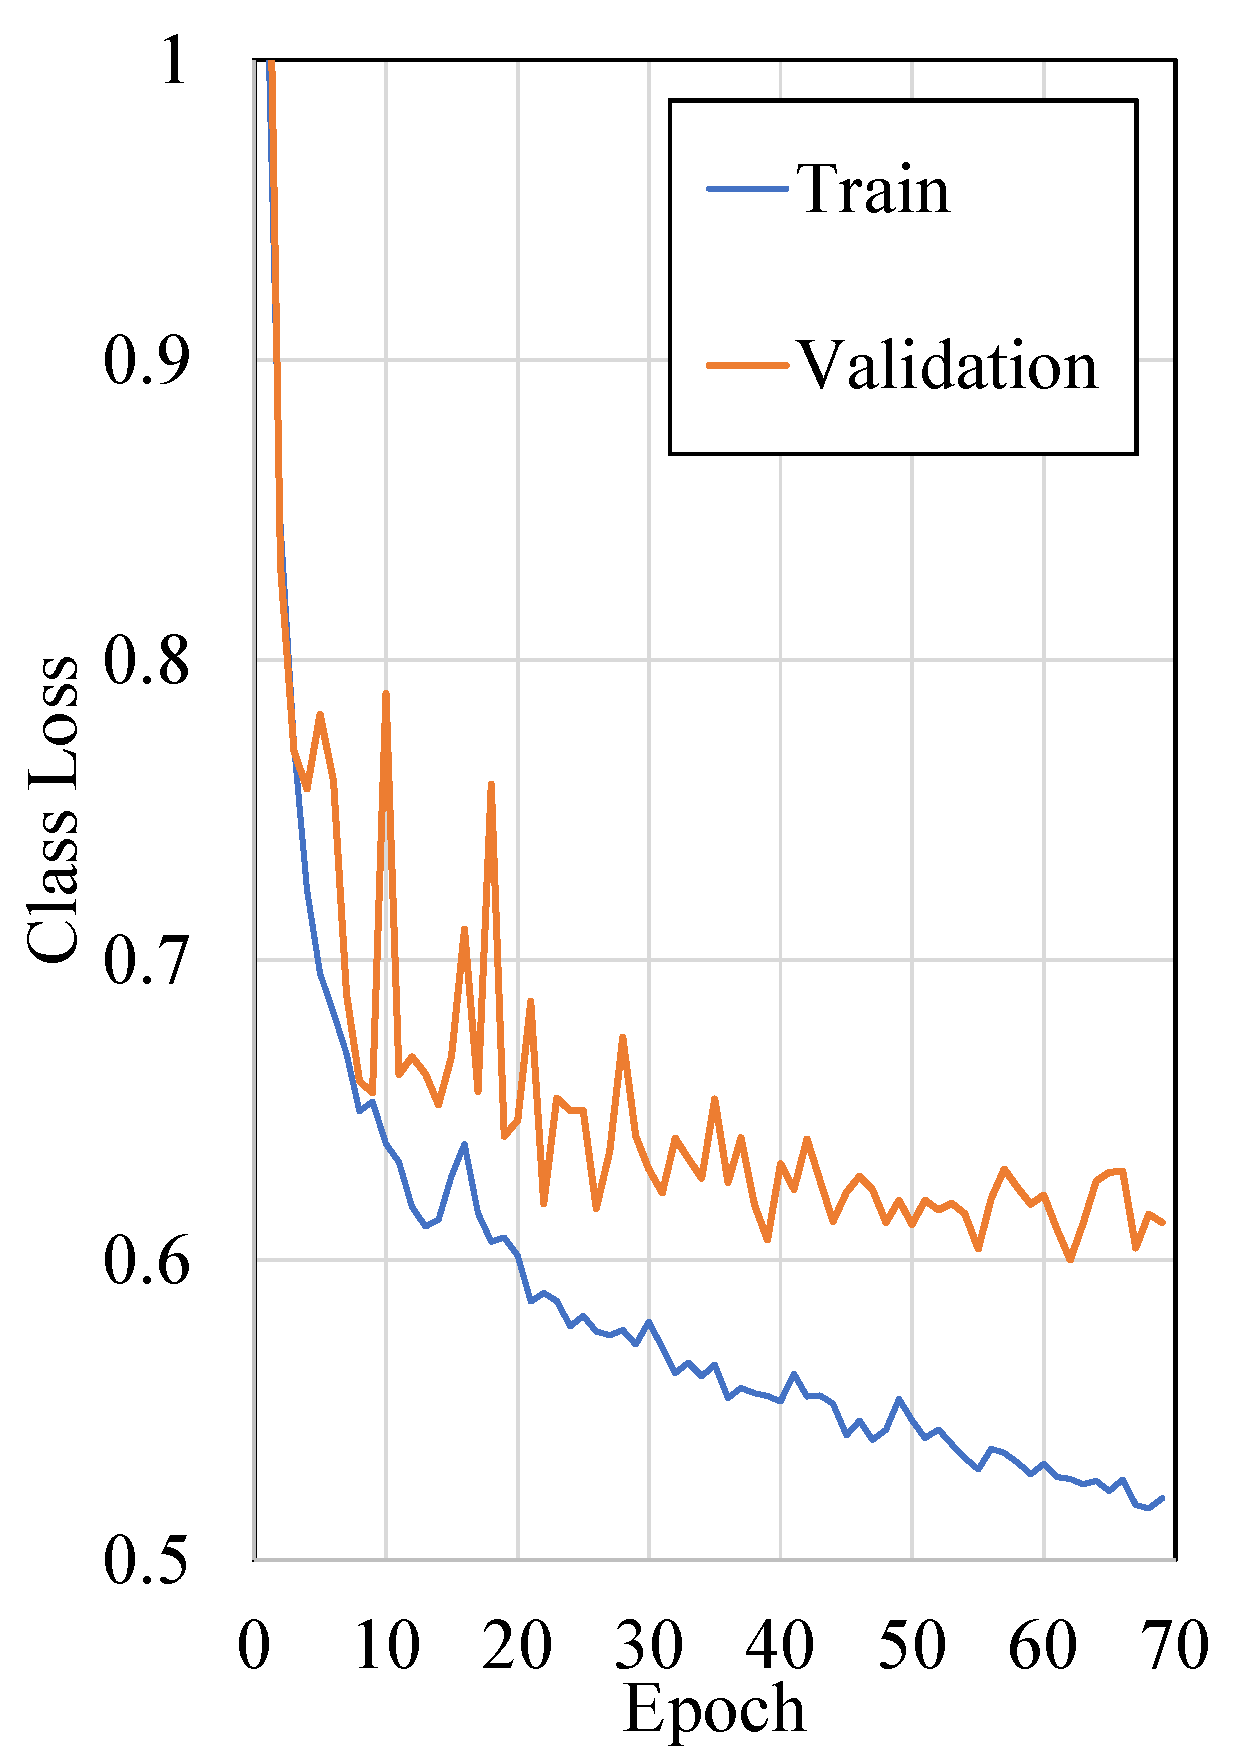
\includegraphics[width=0.333\linewidth]{Images/clss2.pdf}\hfill
  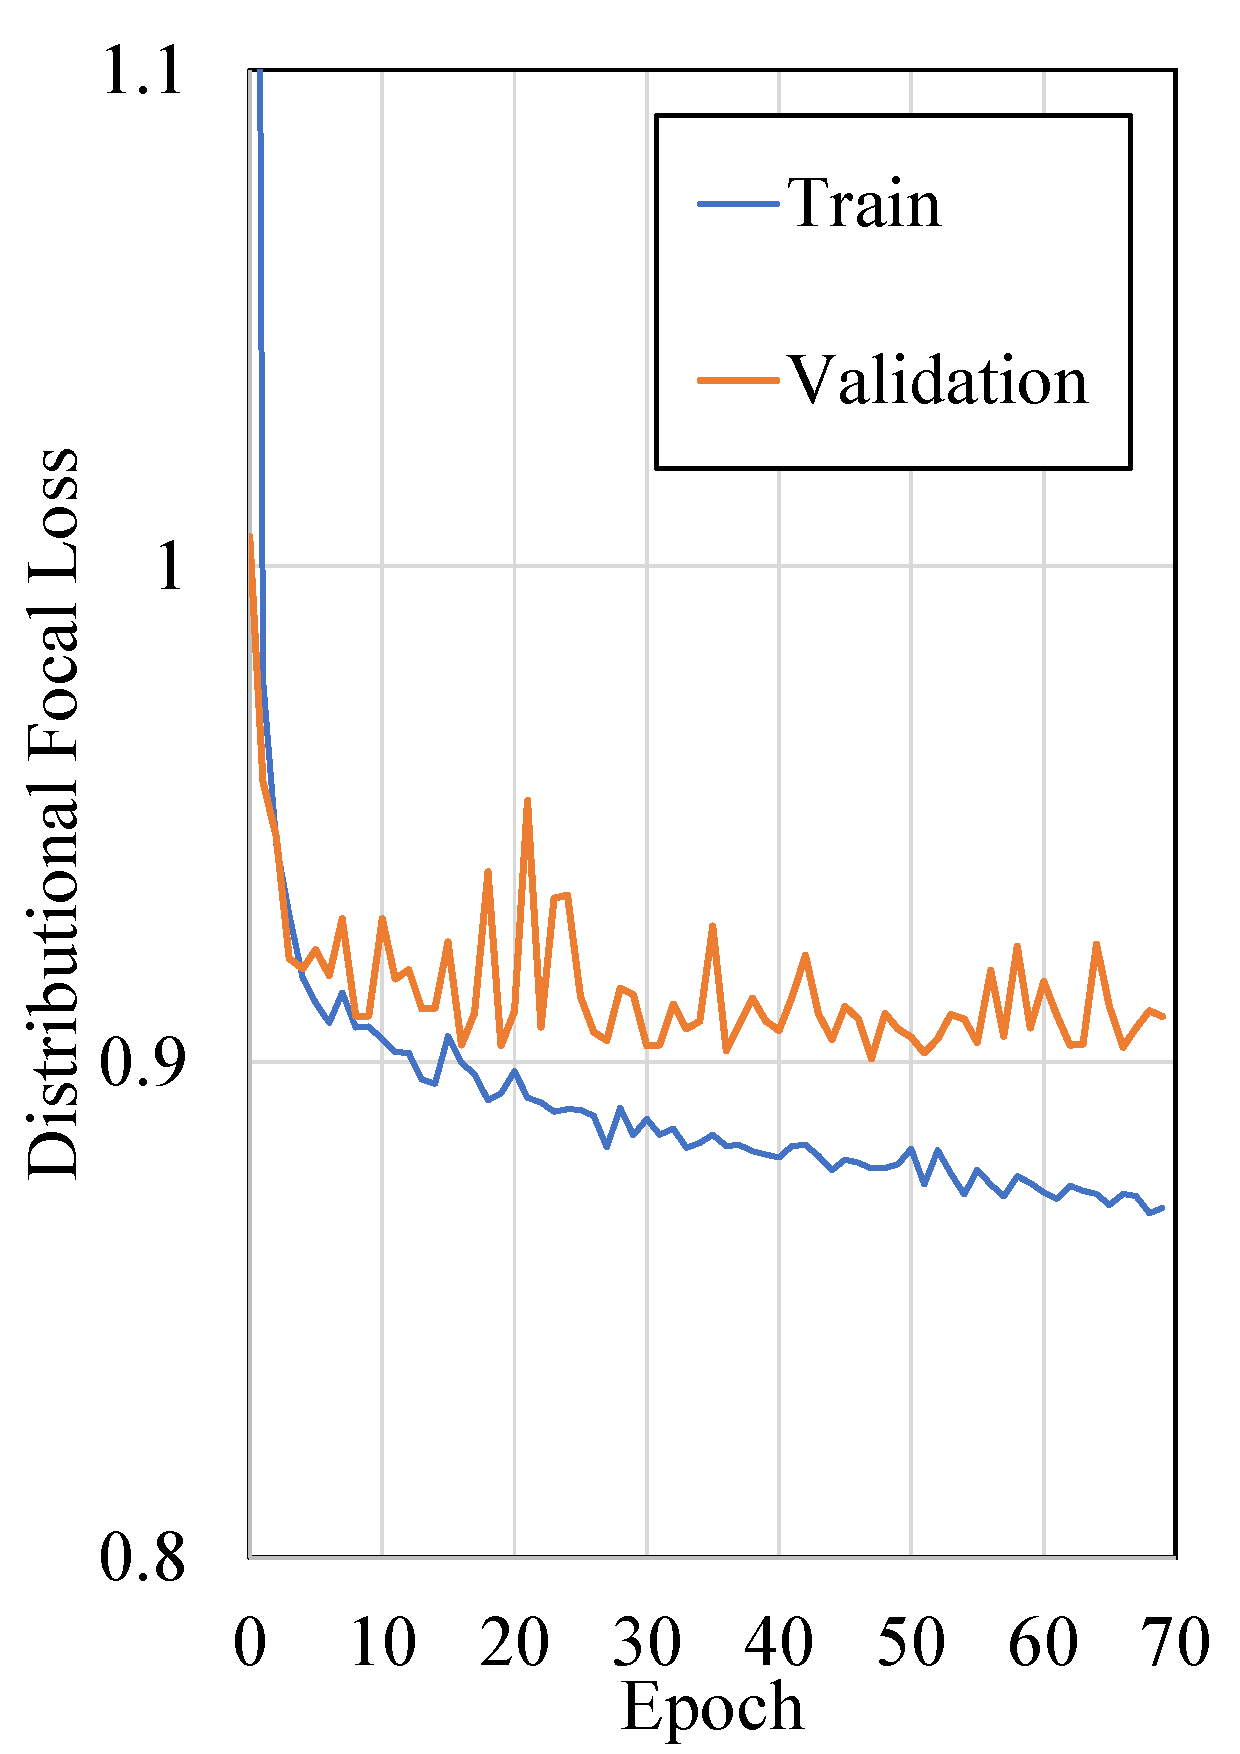
\includegraphics[width=0.333\linewidth]{Images/dfl2.pdf}%
  \end{minipage}%
  \caption{Final Model Train/Validation Comparison}
  \label{final}
\end{figure}

The above figure shows that after a certain number of epochs, the training losses decrease when the training continues. This is from the model overfitting to the training set. If the model continues training after this stage, the accuracy of the model in validation and test sets will degrade. Therefore, although the training was initially planned for 100 epochs, it stopped at 70, and the model at the 50\textsuperscript{th} epoch was extracted to be used. The final results of the model in the train, validation, and test sets are in Table \ref{finaltable}.

\begin{table}[h]
\centering
\begin{tabular}{|cc|cc|cc|}
\hline
\multicolumn{2}{|c|}{\textbf{Train}} & \multicolumn{2}{c|}{\textbf{Validation}} & \multicolumn{2}{c|}{\textbf{Test}} \\ \hline
\multicolumn{1}{|c|}{mAP50} & mAP50-95 & \multicolumn{1}{c|}{mAP50} & mAP50-95 & \multicolumn{1}{c|}{mAP50} & mAP50-95 \\ \hline
\multicolumn{1}{|c|}{97.3\%} & 61.3\% & \multicolumn{1}{c|}{96.8\%} & 54.0\% & \multicolumn{1}{c|}{96.3\%} & 58.7\% \\ \hline
\end{tabular}%
\caption{Final Model Results}
\label{finaltable}
\end{table}

Although the mAP50 of the testing set only increased by 0.3\% from the preliminary training results, the other accuracy metric, mAP 50-95, has increased more than 2\%. That means the overall quality of detection has increased by a margin. 
\newpage
Another way to evaluate the model's performance is by addressing the model's precision and recall. In object detection tasks, precision is how many of the model's detections passed the IOU threshold (i.e., 50\%). Recall means how many ground truths were detected by the model with higher IOUs than the threshold. They are often defined as the following equations:
\begin{equation}
    Precision = \frac{True Positive}{True Positive + False Positive}
    \label{precision}
\end{equation}
\begin{equation}
    Recall = \frac{True Positive}{True Positive + False Nagative}
\end{equation}

In ideal cases, with no false positives or negatives, both numbers become 1. But in real cases, they are often in a trade-off relationship. If the confidence threshold is lowered, the number of false positives will increase, lowering the precision of the model. In contrast, the number of false negatives will decrease, increasing the recall of the model. Because of this relationship, most precision-recall curves form a downward slope. The more reaching the top right corner, the better. Figure \ref{prcurve} shows the precision-recall curve of this model.

\begin{figure}[h]
    \centering
    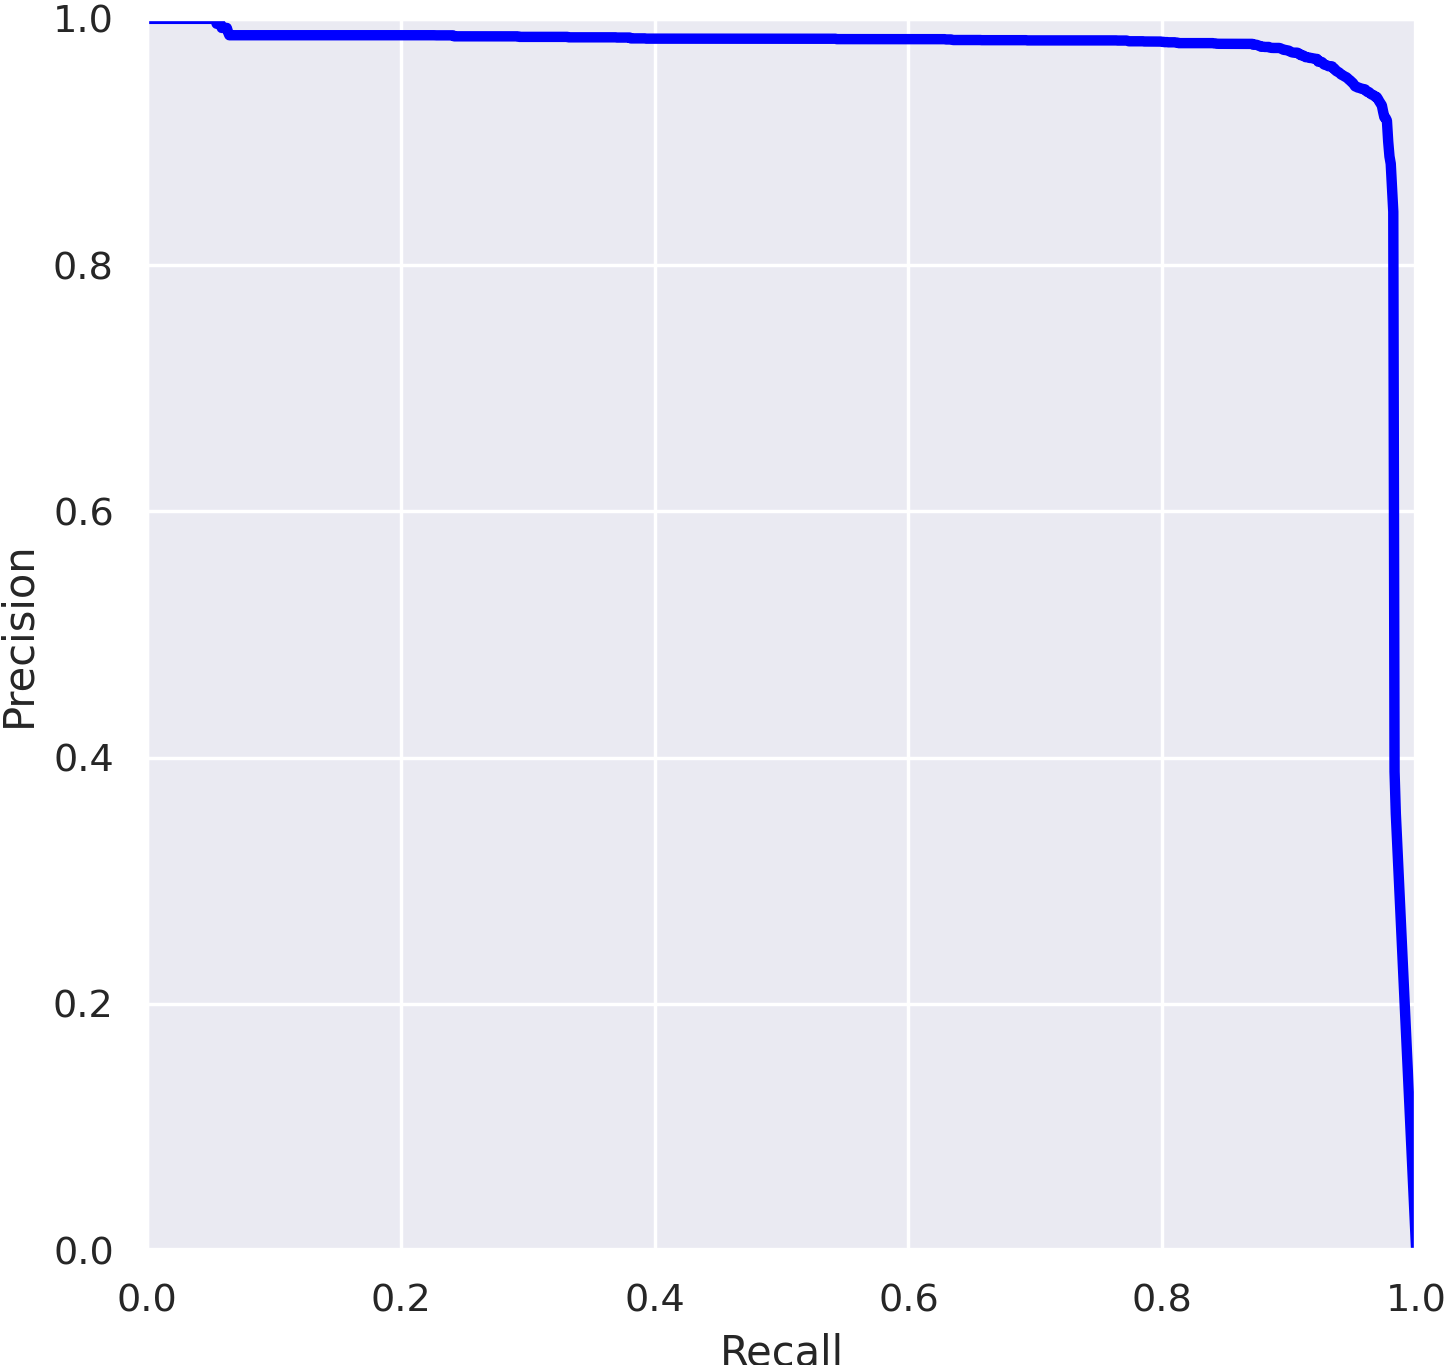
\includegraphics[width=0.7\textwidth]{Images/PR_curve.png}
    \caption{Precision-Recall Curve}
    \label{prcurve}
\end{figure}

Figure \ref{prcurve} shows that this model is robust against false positives and negatives. The model maintains more than 93\% precision and recall through the whole confidence threshold range. Moreover, an F1 score can be calculated to find the optimal confidence threshold for the highest precision and recall simultaneously. The calculation method of the F1 score is as follows.

\begin{equation}
    F1 Score = \frac{2 \times (Precision \times Recall)}{Precision+Recall}
    \label{f1score}
\end{equation}

Then, a graph can be plotted for F1 scores against different confidence values. 

\begin{figure}[h]
    \centering
    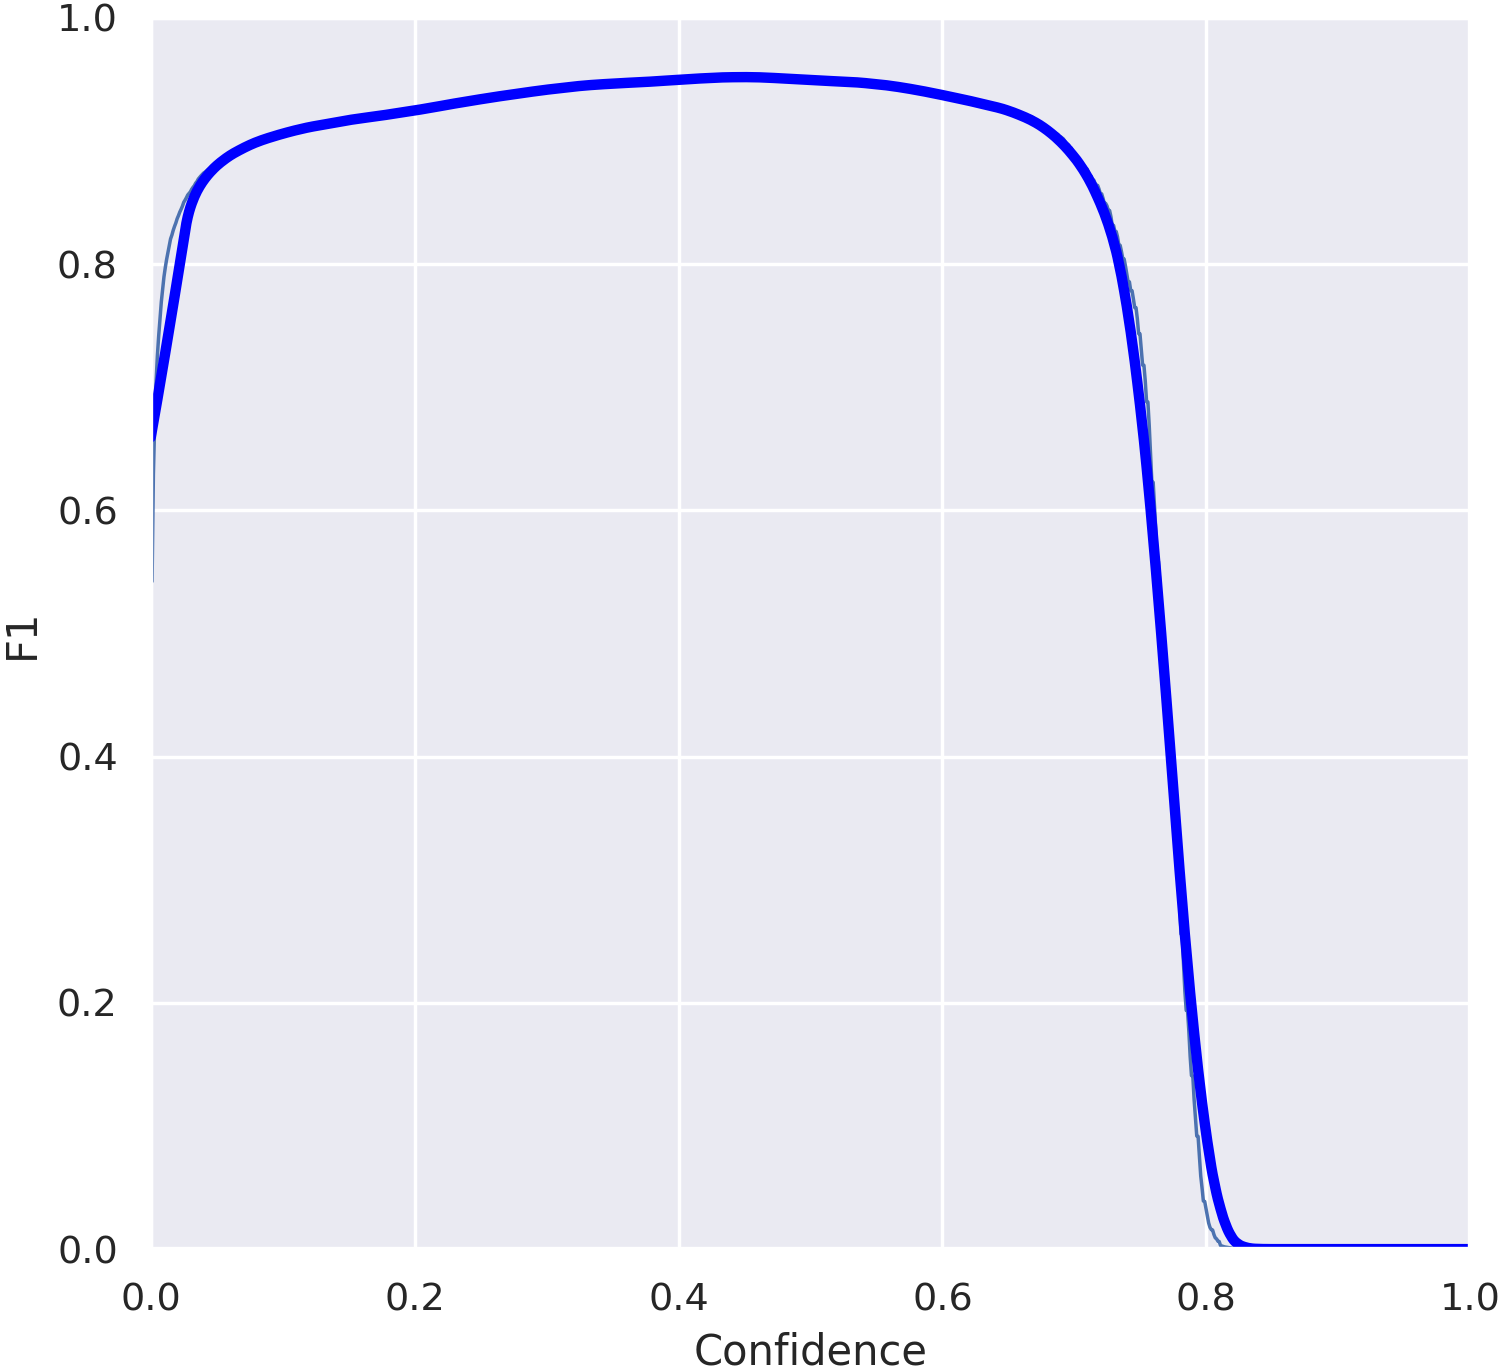
\includegraphics[width=0.7\textwidth]{Images/F1_curve.png}
    \caption{F1-Confidence Curve}
    \label{f1curve}
\end{figure}

Figure \ref{f1curve} shows the optimal confidence value of 0.45. This value will be used for the model during the tracking process.

The following figures are the prediction results from the model in the validation and test sets. Along with the detection, there are the class name and the confidence score. 

\begin{figure}
    \centering
    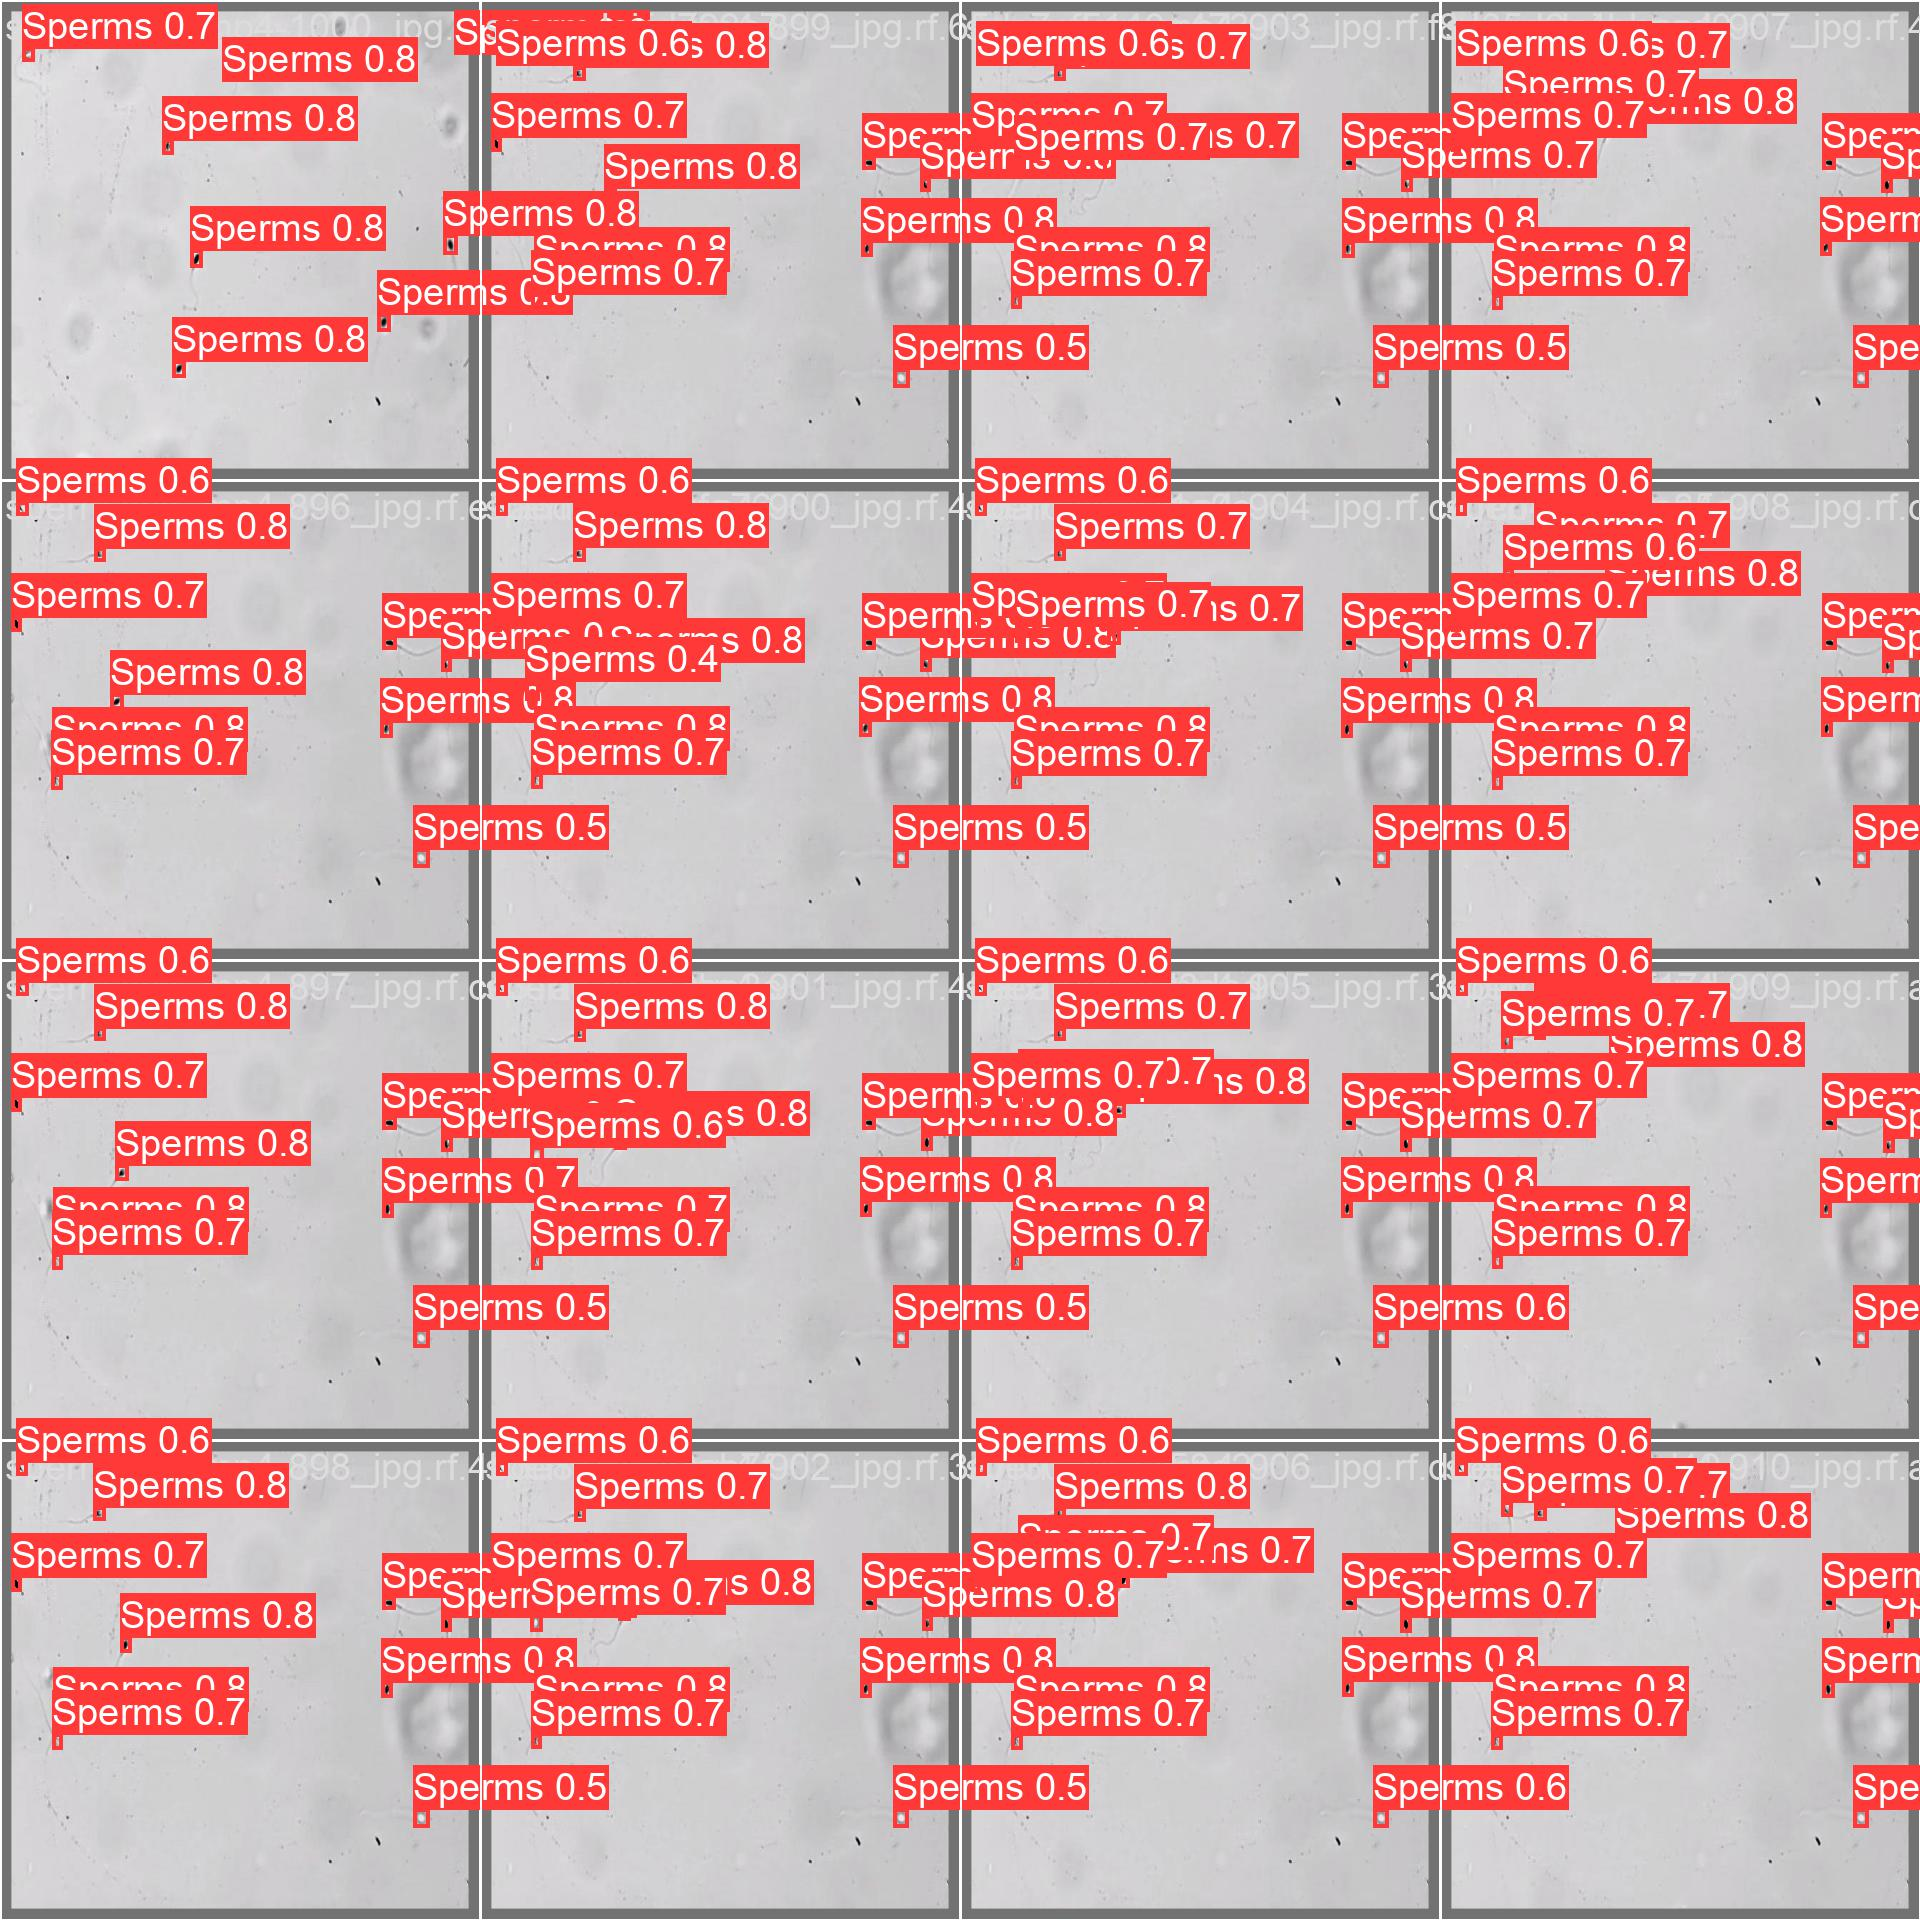
\includegraphics[width=\textwidth]{Images/val_batch0_pred.jpg}
    \caption{Validation Set Prediction}
    \label{valpred}
\end{figure}

\begin{figure}
    \centering
    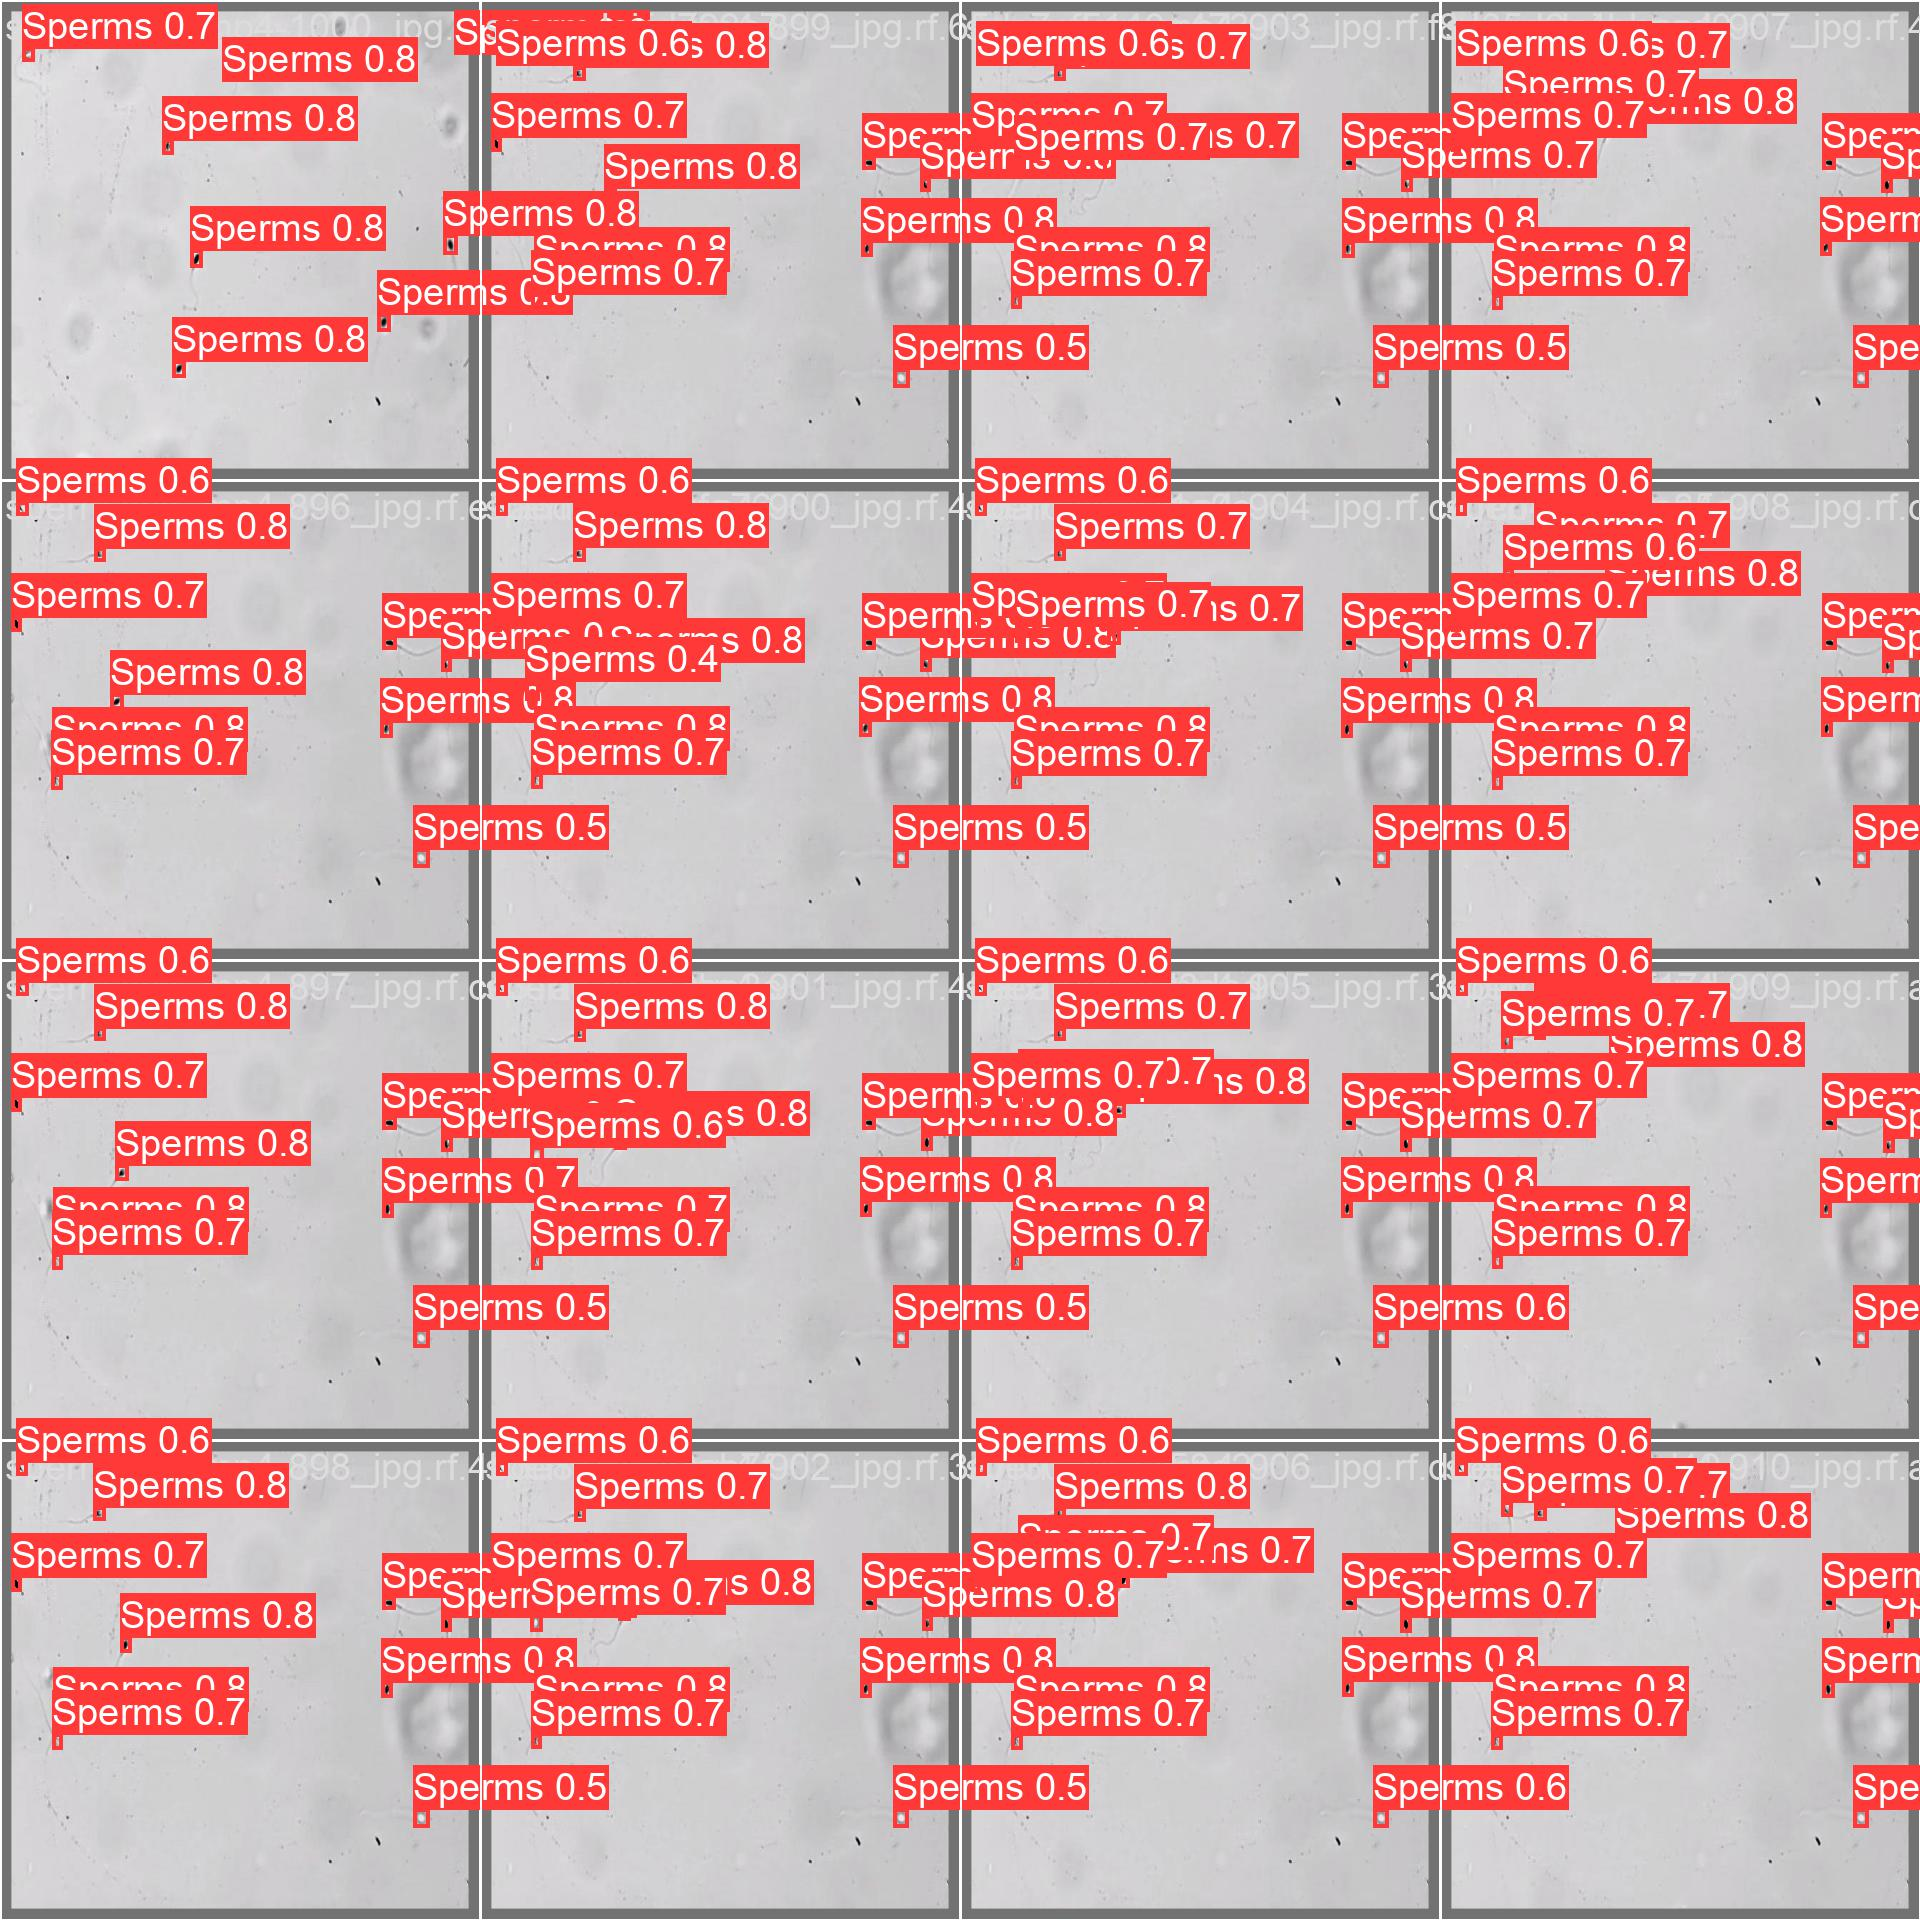
\includegraphics[width=\textwidth]{Images/val_batch0_pred (1).jpg}
    \caption{Test Set Prediction}
    \label{testpred}
\end{figure}
\newpage
\section{Tracking Result}
Five video samples with different characteristics were extracted to test this program's tracking function. The first three samples had high, medium, and low counts of sperms. These three samples will evaluate the performance of the tracking program in situations with different probabilities of occlusion, as more sperms will lead to more crossing-overs between them. Moreover, this will test the program's ability to handle real-time tracking since more calculations will be needed for more sperms. Figure \ref{sam1-3} shows the snapshot of each sample. 

\begin{figure}[h]
     \centering
     \begin{subfigure}[b]{0.31\textwidth}
         \centering
         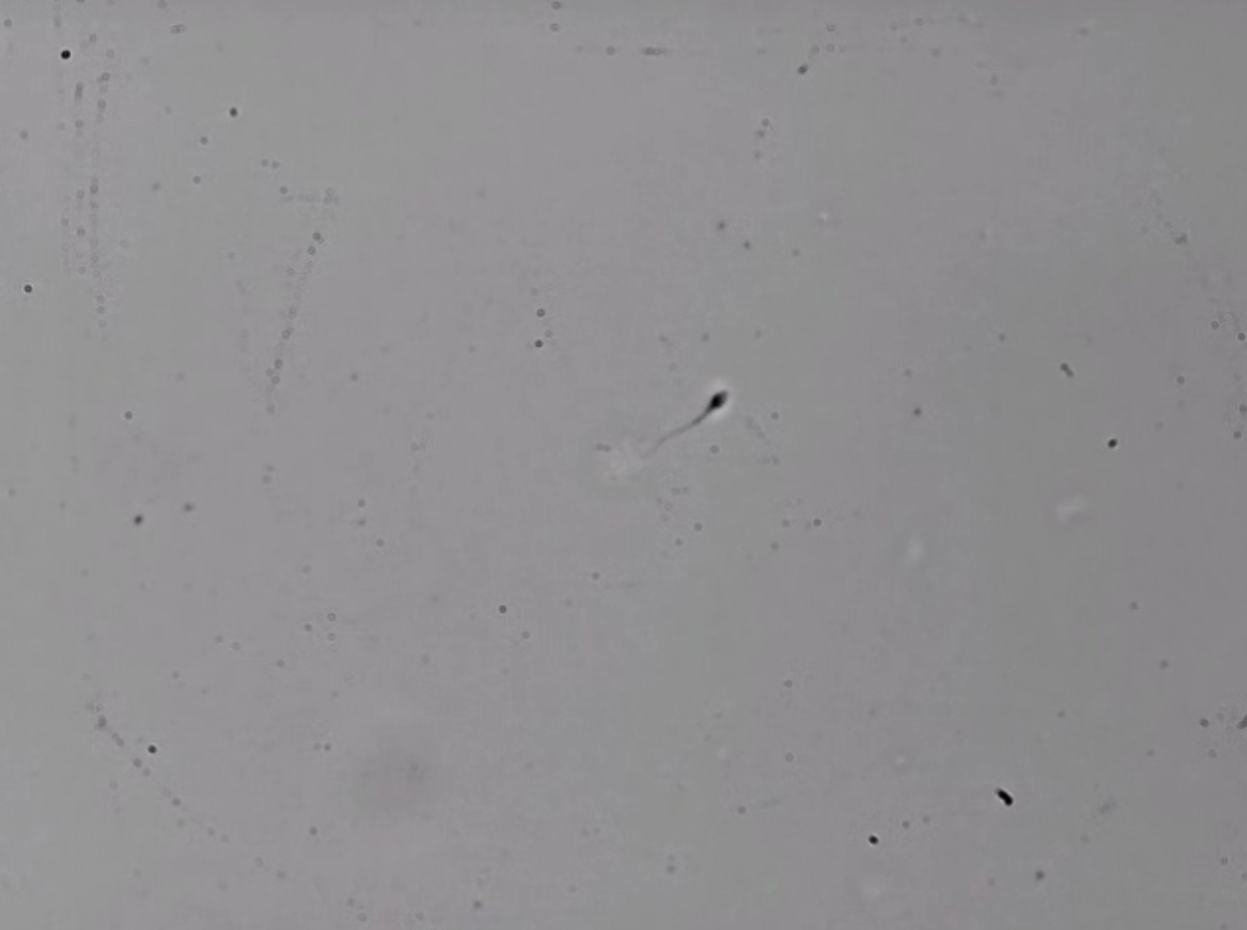
\includegraphics[width=\textwidth]{Images/low.png}
         \caption{Sample 1: Low}
         \label{sam1}
     \end{subfigure}
     \hfill
     \begin{subfigure}[b]{0.31\textwidth}
         \centering
         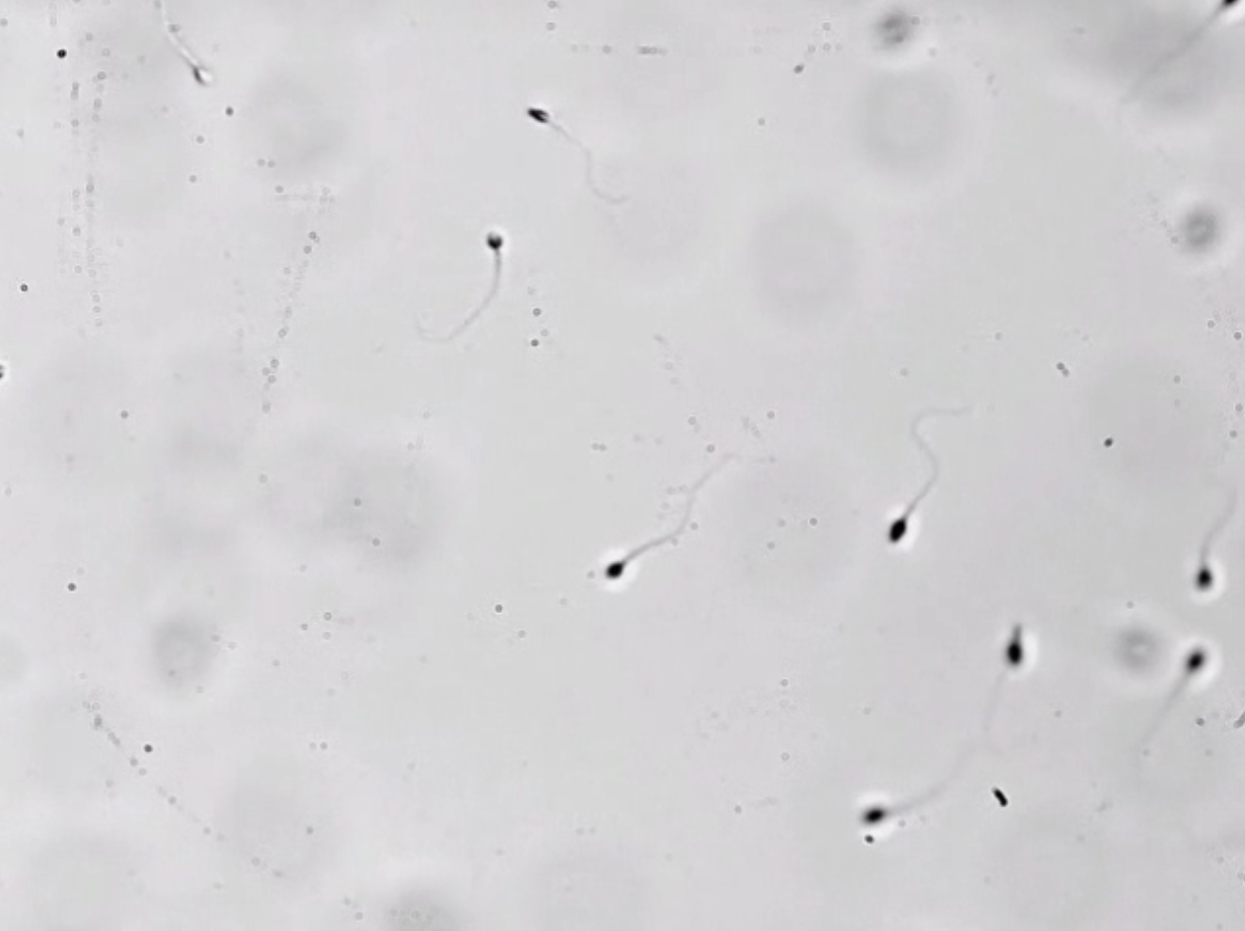
\includegraphics[width=\textwidth]{Images/med.png}
         \caption{Sample 2: Medium}
         \label{sam2}
     \end{subfigure}
     \hfill
     \begin{subfigure}[b]{0.31\textwidth}
         \centering
         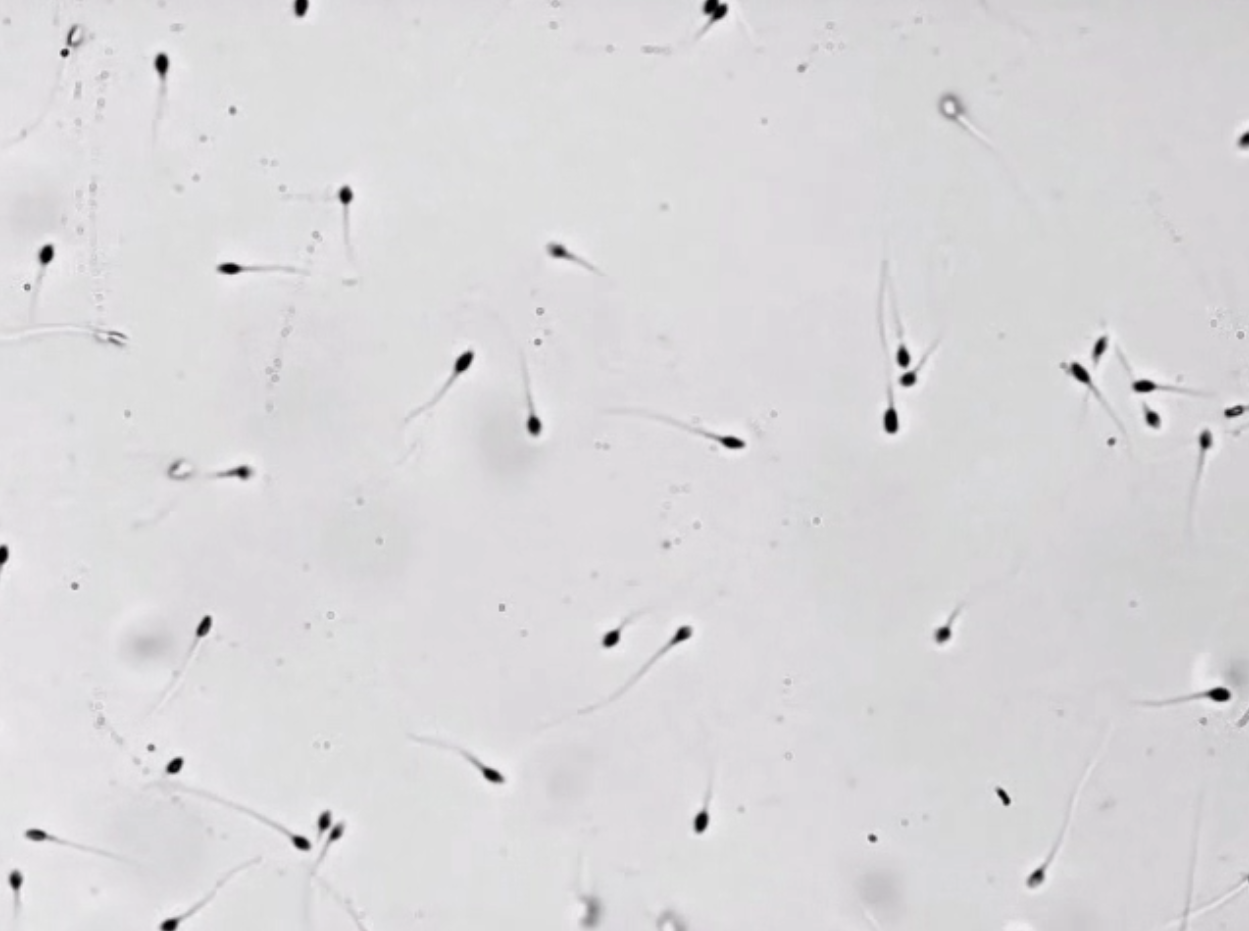
\includegraphics[width=\textwidth]{Images/high.png}
         \caption{Sample 3: High}
         \label{sam3}
     \end{subfigure}
        \caption{Tracking Samples 1-3}
        \label{sam1-3}
\end{figure}

The remaining two samples will test the program's robustness to blurry sperms. The program will be particularly examined for its ability to detect and track blurry sperms and its capacity to predict the tracks of blurry sperms when it is undetected by the model for multiple frames. Figure \ref{sam4-5} shows the snapshot of the last two testing samples.

\begin{figure}[h]
     \centering
     \begin{subfigure}[b]{0.46\textwidth}
         \centering
         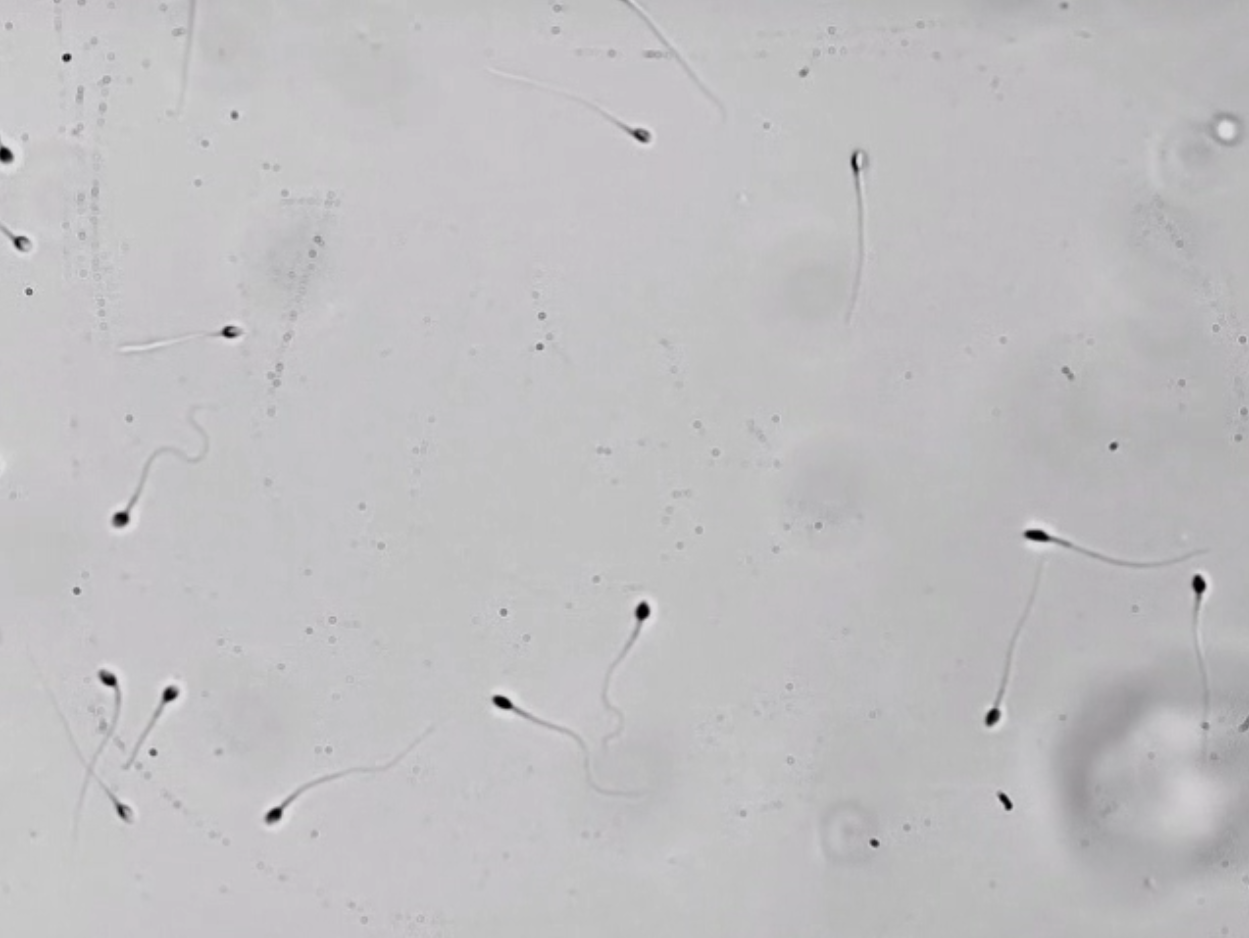
\includegraphics[width=\textwidth]{Images/clear.png}
         \caption{Sample 4: Clear}
         \label{sam4}
     \end{subfigure}
     \hfill
     \begin{subfigure}[b]{0.46\textwidth}
         \centering
         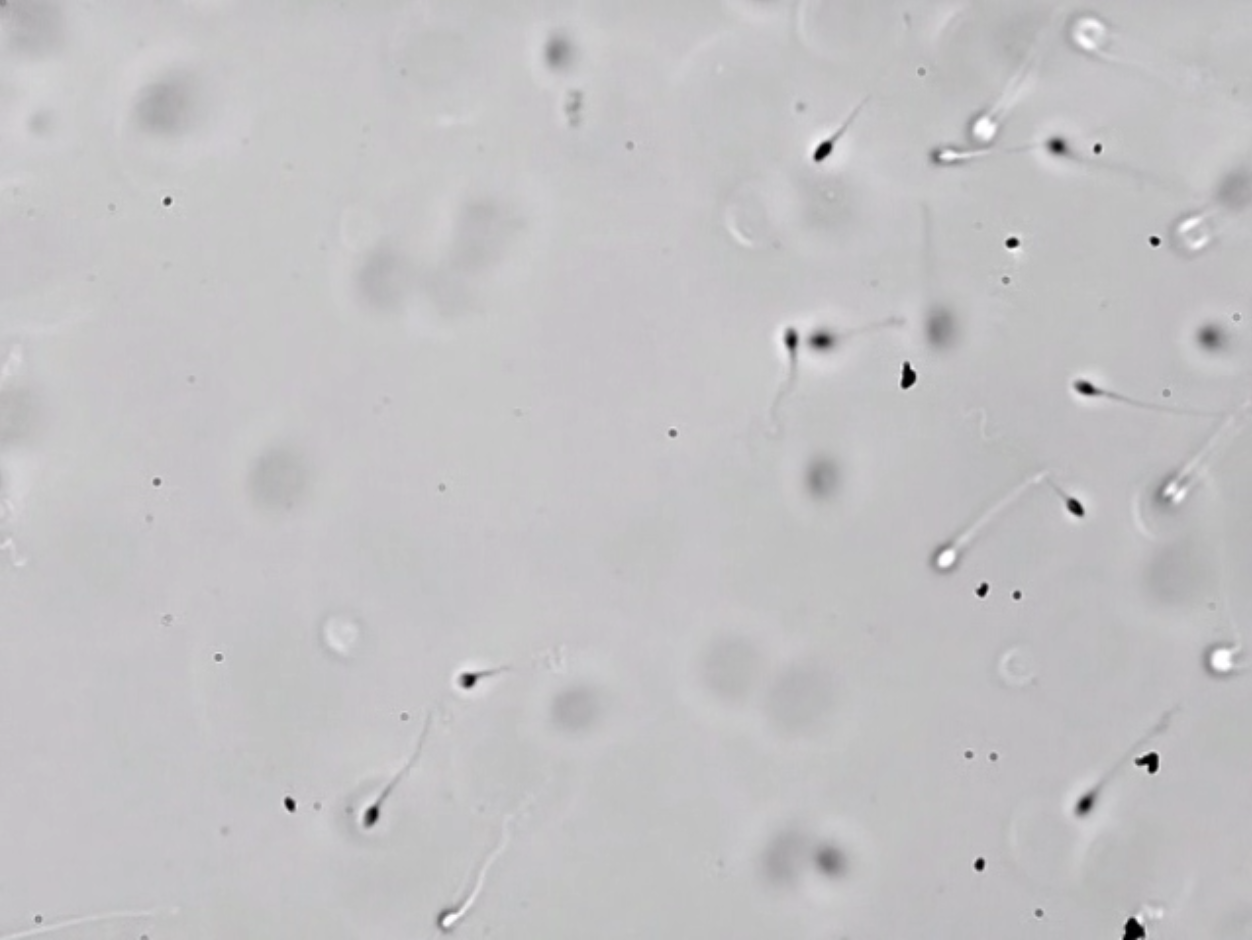
\includegraphics[width=\textwidth]{Images/blurry.png}
         \caption{Sample 5: Blurry}
         \label{sam5}
     \end{subfigure}
        \caption{Tracking Samples 4-5}
        \label{sam4-5}
\end{figure}
The sample videos and the program output videos are available at \href{https://github.com/rladntjr7/FYP}{\underline{GitHub}}.


As shown in Figure \ref{sam4-5}, Sample 4 has the sperms that clearly indicate the sperm heads. Whereas Sample 5 contains many sperms that appear not as clearly as those from Sample 4. It can be speculated that those sperms that are not perfectly focused from the camera appear white and round. As shown in Figure \ref{valpred} and  Figure \ref{testpred}, these kinds of sperms tend to have lower confidence scores than those with more clear shapes. This will lead to those sperms intermittently detected by the model, testing the occlusion tracking function. 

\subsubsection{Sample 1: Low Count}
Figure \ref{sam1res} shows the snapshot of the program output of sample 1. 
\begin{figure}[h]
    \centering
    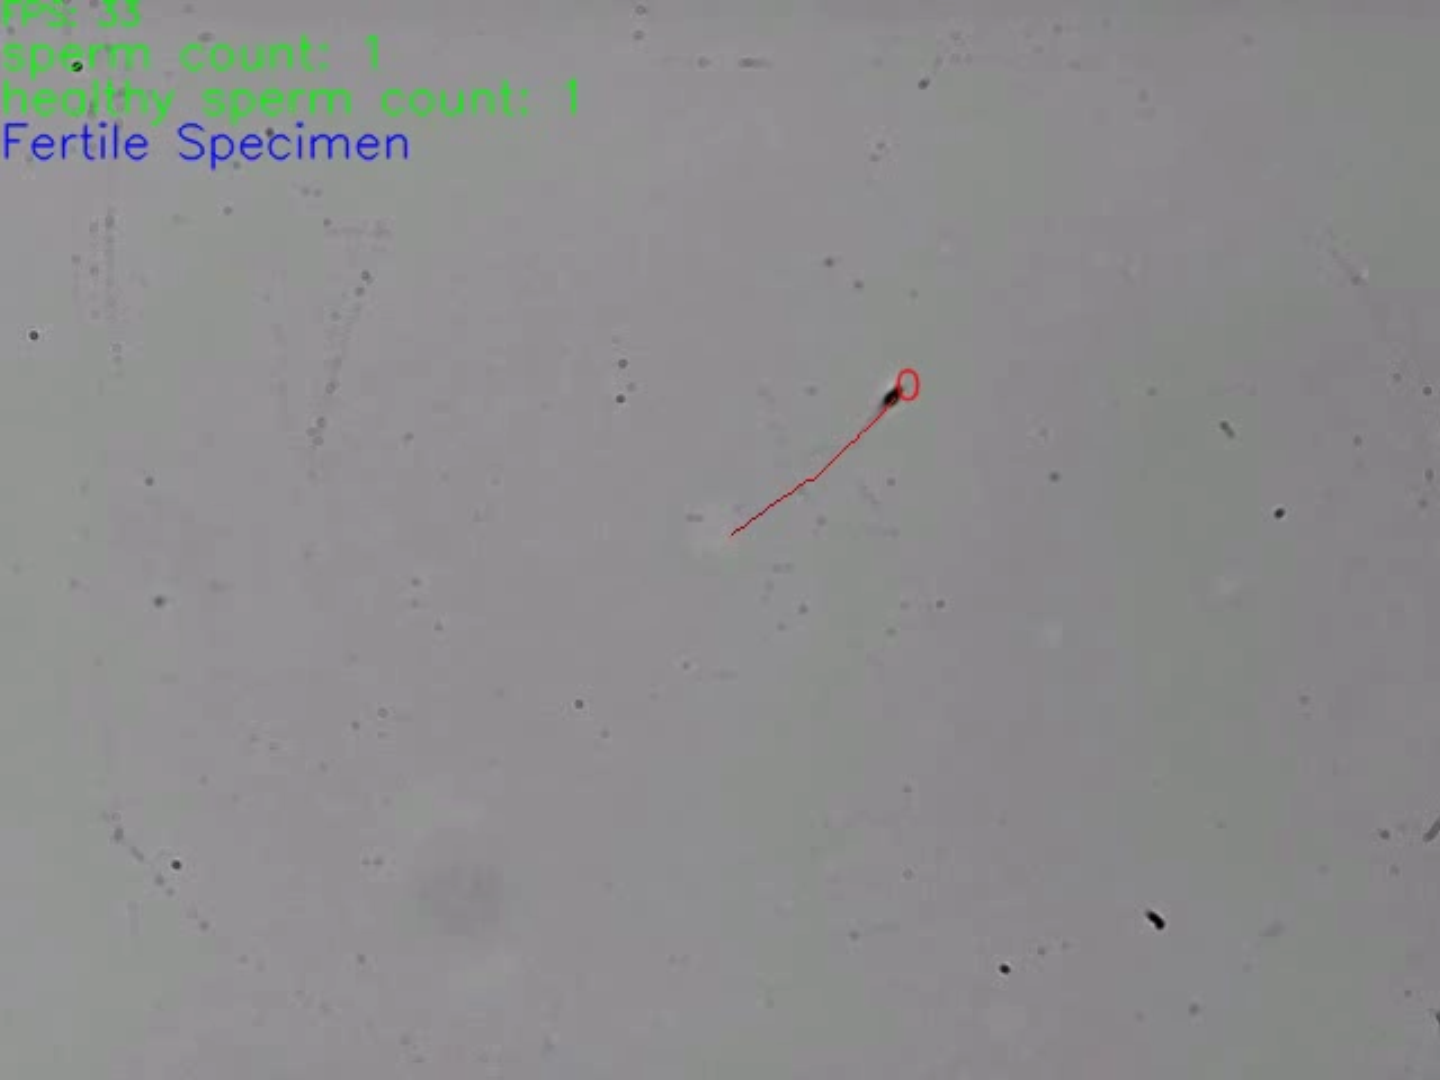
\includegraphics[width=0.75\textwidth]{Images/sam1.png}
    \caption{Sample 1 Output}
    \label{sam1res}
\end{figure}

With one sperm, the model had a satisfactory result. The FPS was over 30 throughout the video, and the ID number correctly followed the sperm head without any ID switch. 

\newpage
\subsubsection{Sample 2: Medium Count}
Figure \ref{sam2res} shows the snapshot of the program output of sample 2.
\begin{figure}[h]
    \centering
    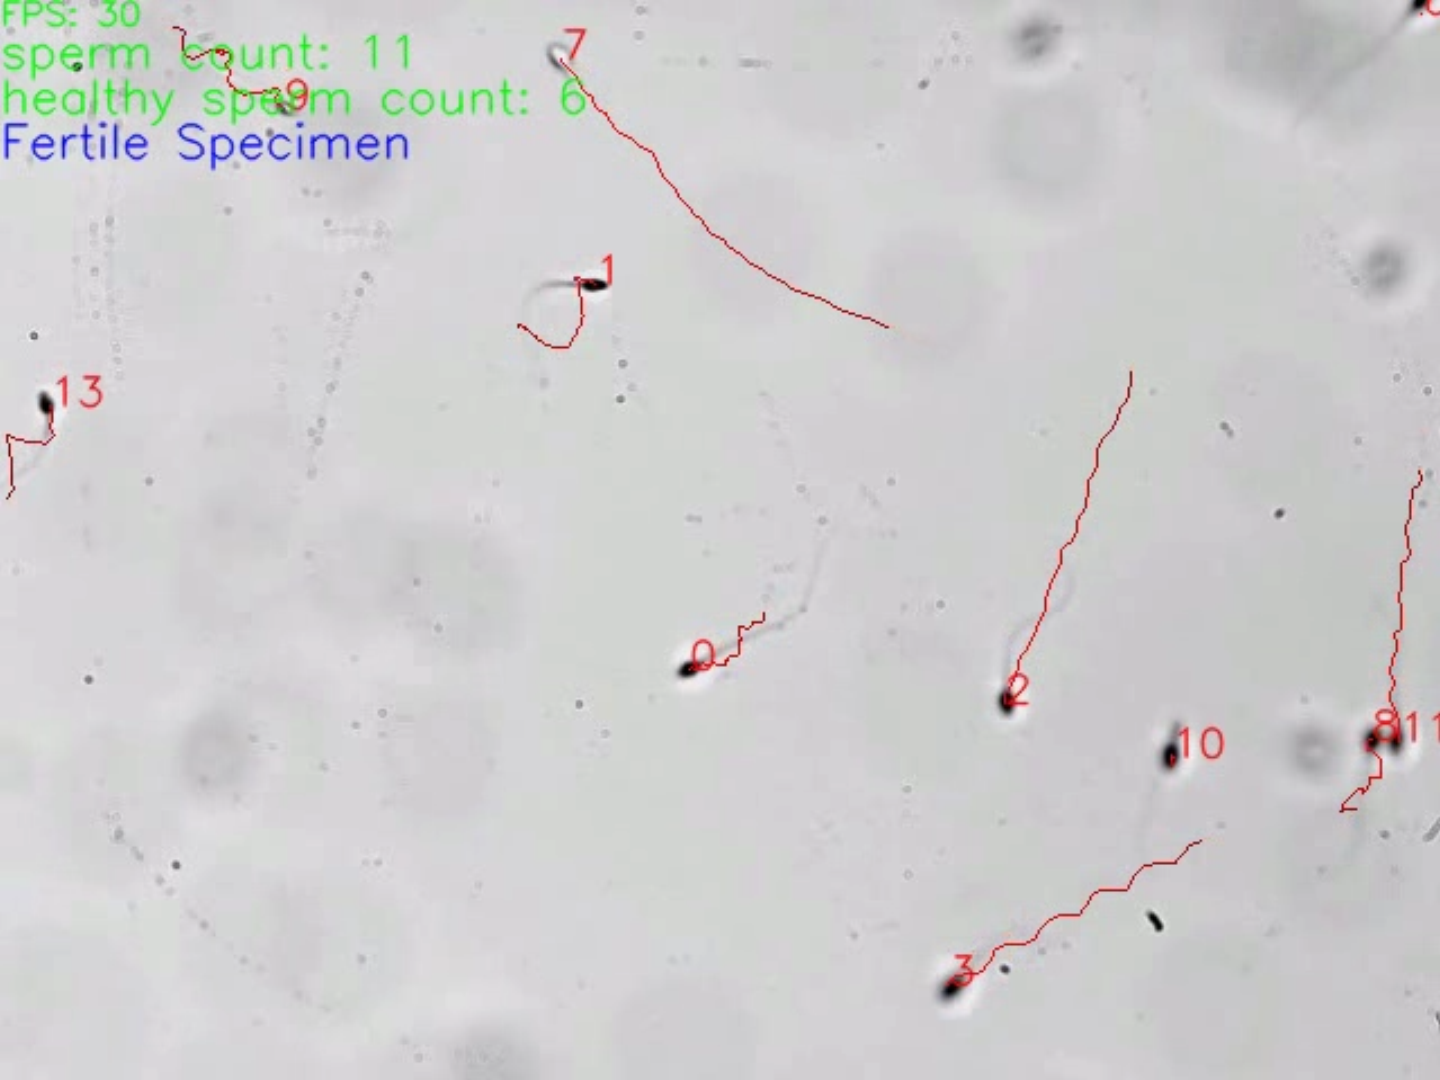
\includegraphics[width=0.75\textwidth]{Images/sam2.png}
    \caption{Sample 2 Output}
    \label{sam2res}
\end{figure}

With multiple sperms in one frame, the program also had a satisfactory result, maintaining 30 frames per second. On the right of Figure \ref{sam2res}, sperm 8 and 11 were moving very closely with each other, but there was no ID switch between them. Moreover, the program deals well with the complex trajectory of sperm 1 and 13, as shown in Figure \ref{sam22}.
\begin{figure}[h]
     \centering
     \begin{subfigure}[b]{0.35\textwidth}
         \centering
         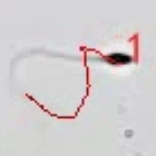
\includegraphics[width=\textwidth]{Images/sam222.png}
     \end{subfigure}
     \hspace{4em}%
     \begin{subfigure}[b]{0.35\textwidth}
         \centering
         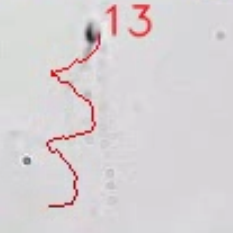
\includegraphics[width=\textwidth]{Images/sam22.png}
     \end{subfigure}
        \caption{Trajectories of Sperm 1 and 13 in Sample 2}
        \label{sam22}
\end{figure}
\newpage
\subsubsection{Sample 3: High Count}
Figure \ref{sam3res} shows the snapshot of the program output of sample 3.
\begin{figure}[h]
    \centering
    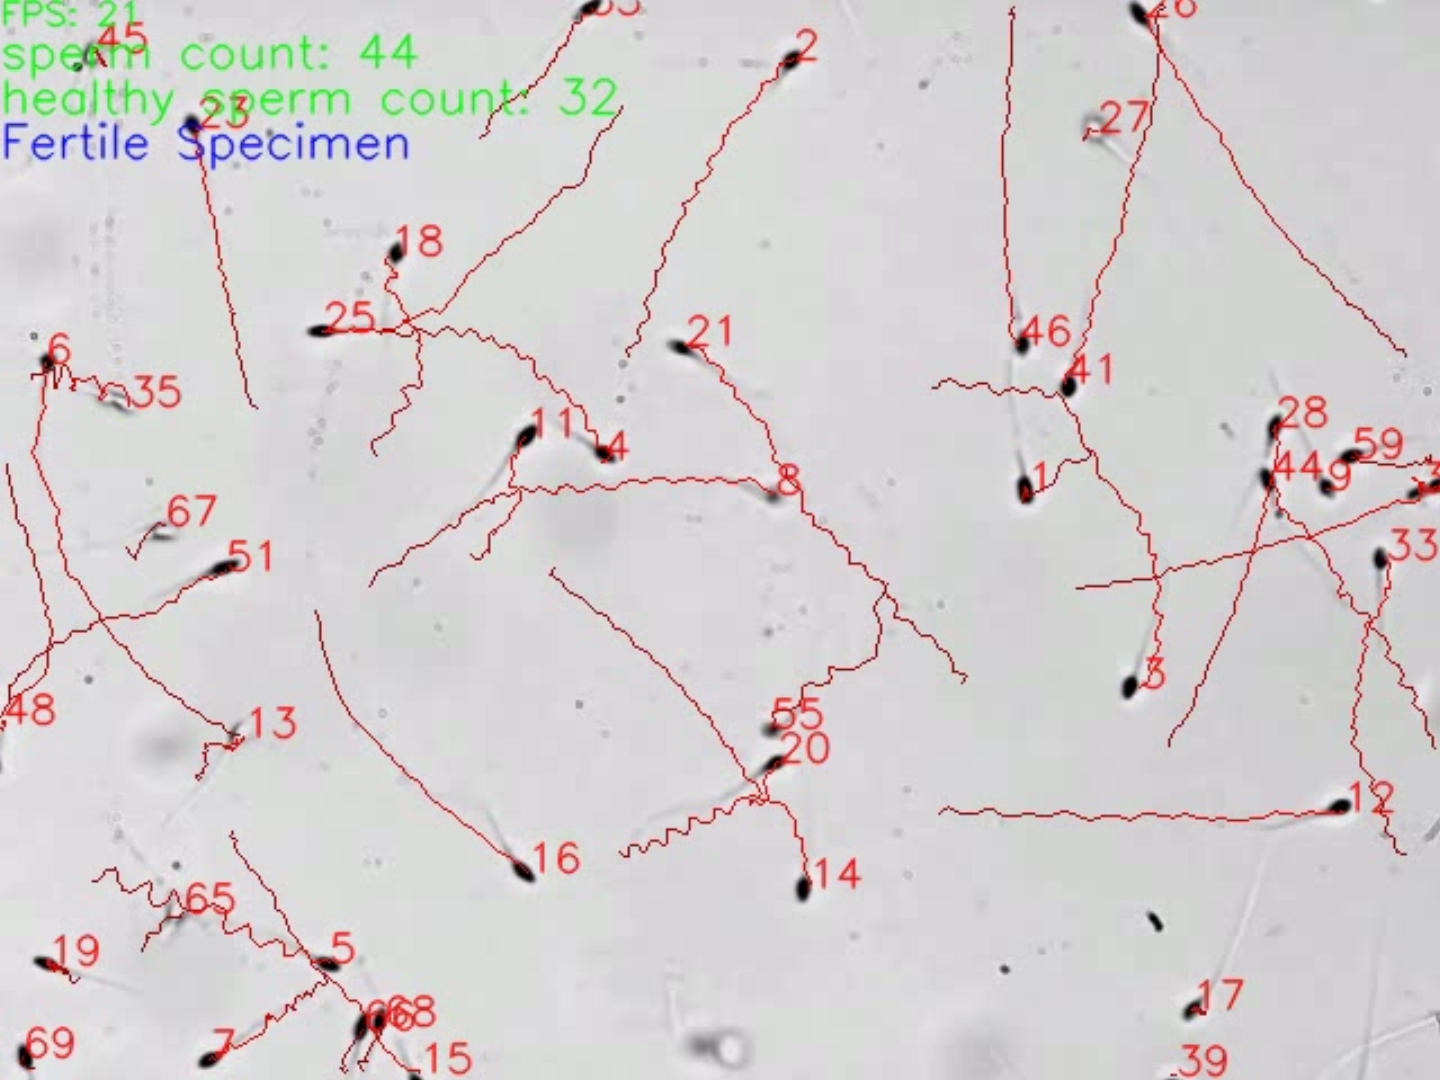
\includegraphics[width=0.75\textwidth]{Images/sam3.png}
    \caption{Sample 3 Output}
    \label{sam3res}
\end{figure}

With many sperms in one frame, the FPS slowed significantly to 20. Also, many collisions and cross-overs were taking place. The model handled some very well, as shown in Figure \ref{sam3col}.
\begin{figure}[h]
     \centering
     \begin{subfigure}[b]{0.34\textwidth}
         \centering
         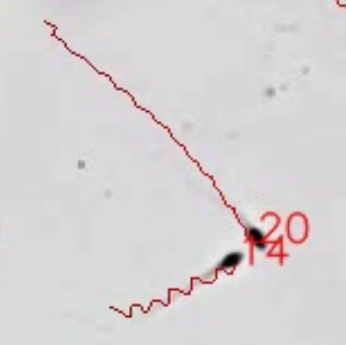
\includegraphics[width=\textwidth]{Images/sam33.png}
     \end{subfigure}
     \hspace{4em}%
     \begin{subfigure}[b]{0.34\textwidth}
         \centering
         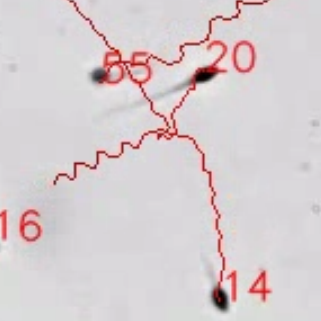
\includegraphics[width=\textwidth]{Images/sam333.png}
     \end{subfigure}
        \caption{Cross-Over of Sperm 14 and 20 in Sample 3}
        \label{sam3col}
\end{figure}

Sperms 14 and 20 had a cross-over, but the program calculated the most probable trajectories of each sperm, and no ID switching occurred.
\newpage
Although not many, ID switching was still occurring due to the rapid movement and collisions of sperms. 

\begin{figure}[ht]
     \centering
     \begin{subfigure}[b]{0.3\textwidth}
         \centering
         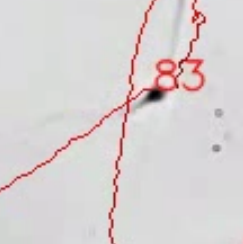
\includegraphics[width=\textwidth]{Images/sam3333.png}
     \end{subfigure}
     \hfill
     \begin{subfigure}[b]{0.3\textwidth}
         \centering
         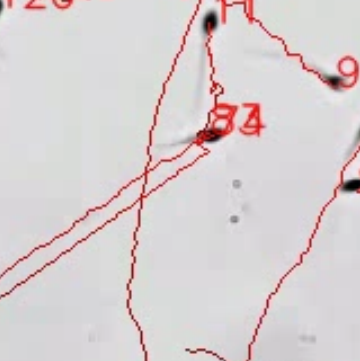
\includegraphics[width=\textwidth]{Images/sam33333.png}
     \end{subfigure}
     \hfill
     \begin{subfigure}[b]{0.3\textwidth}
         \centering
         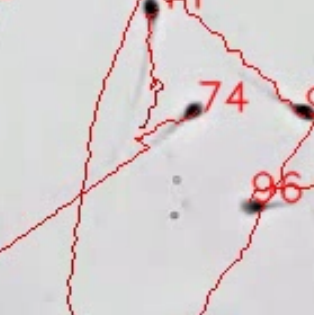
\includegraphics[width=\textwidth]{Images/sam333333.png}
     \end{subfigure}
        \caption{ID Switching of Sperm 83 to 74 in Sample 3}
        \label{sam3sw}
\end{figure}

In Figure \ref{sam3sw}, Sperm 83 was switched to 74. The cause of this switching is track 74 not being permanently disabled after it becomes inactive. Then, the detection at a certain frame was closer to track 74 than its original track, and it switched the ID.

\begin{figure}[h]
     \centering
     \begin{subfigure}[b]{0.3\textwidth}
         \centering
         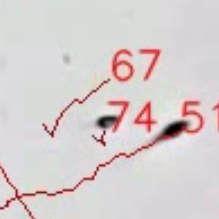
\includegraphics[width=\textwidth]{Images/sam3333333.png}
         \caption{67 \textrightarrow 74}
     \end{subfigure}
     \hfill
     \begin{subfigure}[b]{0.3\textwidth}
         \centering
         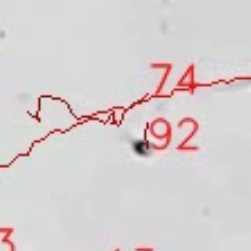
\includegraphics[width=\textwidth]{Images/sam33333333.png}
         \caption{74 \textrightarrow 92}
     \end{subfigure}
     \hfill
     \begin{subfigure}[b]{0.3\textwidth}
         \centering
         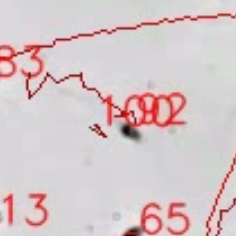
\includegraphics[width=\textwidth]{Images/sam333333333.png}
         \caption{92 \textrightarrow 100}
     \end{subfigure}
        \caption{Sperm with Multiple IDs Assigned in Sample 3}
        \label{sam3mult}
\end{figure}

Figure \ref{sam3mult} shows a sperm assigned to multiple IDs. The sperm's original ID was 56, but whenever it made a sharp turn, the program could not follow the correct trajectory and assigned a new ID. 

These issues do not degrade the model's overall performance significantly because most of the sperms are working well. Still, it can be improved for the quality of the program.

\newpage
\subsubsection{Sample 4: Clear Sperms}
Figure \ref{sam4res} shows the snapshot of the program output of sample 4.
\begin{figure}[h]
    \centering
    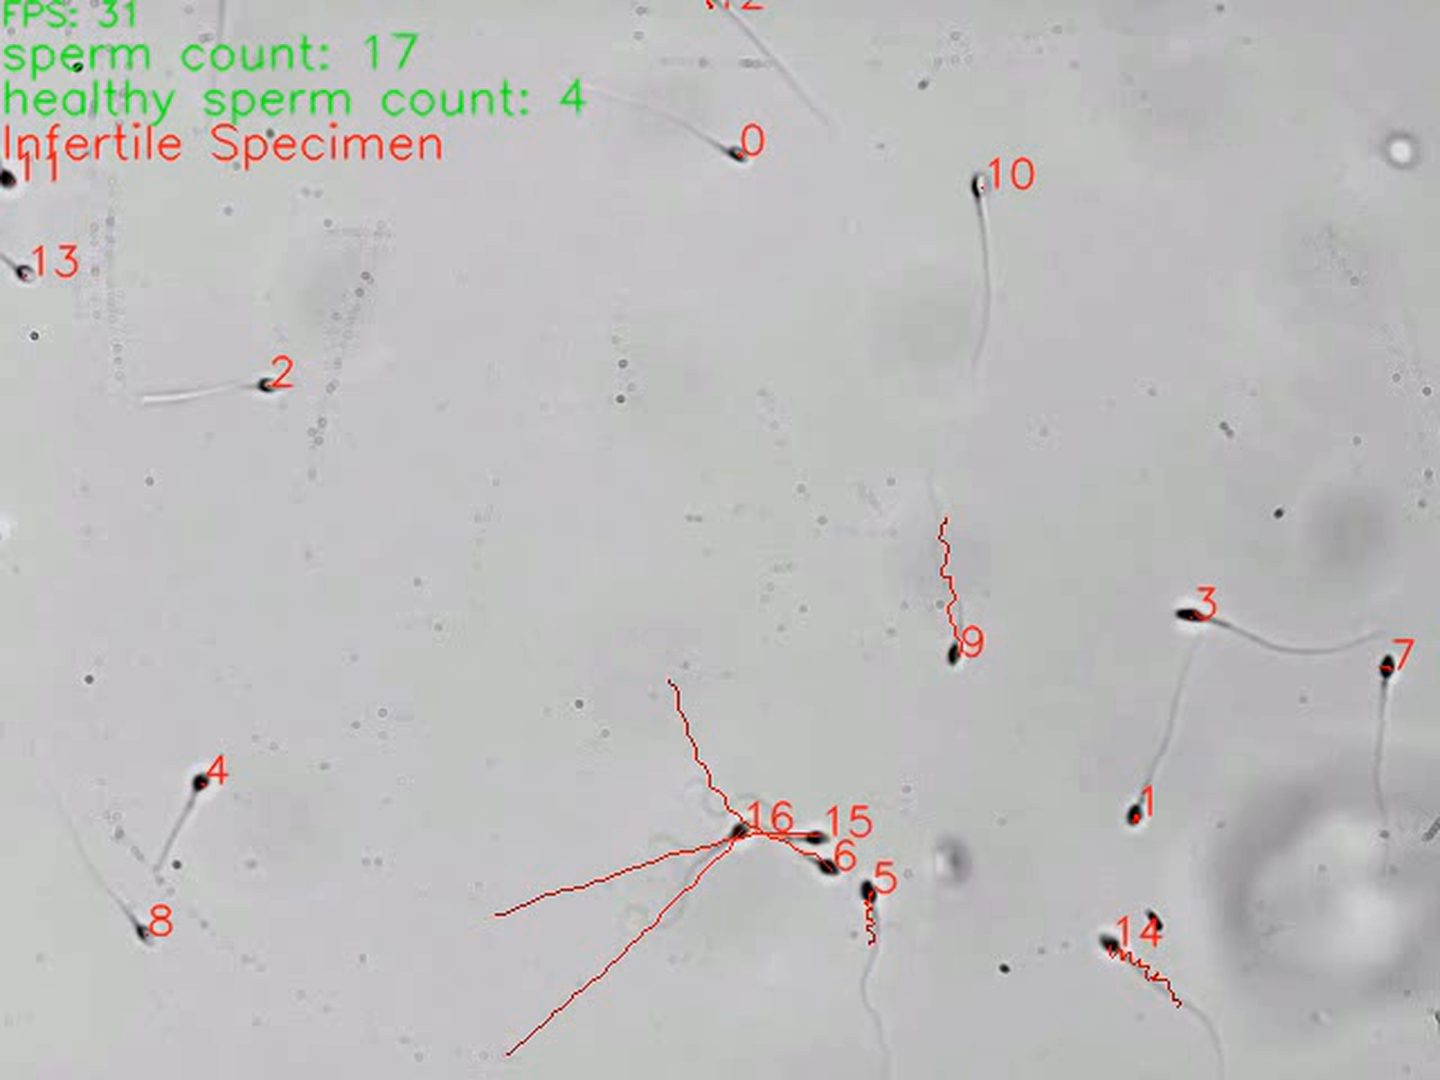
\includegraphics[width=0.75\textwidth]{Images/sam4.png}
    \caption{Sample 4 Output}
    \label{sam4res}
\end{figure}

With clear images, the model's performance was satisfactory. Having relatively fewer sperms, the FPS was well maintained above 30, and the infertility status of the specimen was correctly assessed. Moreover, it dealt with the cross-over of 3 sperms at the same time very well, as shown in Figure \ref{sam4cross}
\begin{figure}[h]
    \centering
    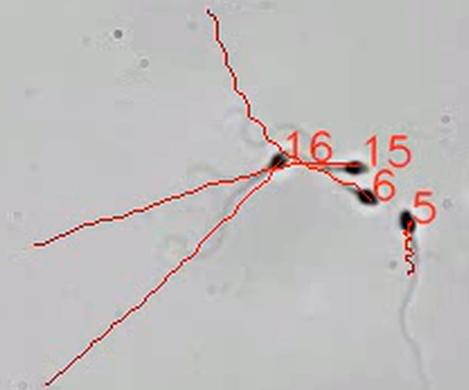
\includegraphics[width=0.42\textwidth]{Images/sam44.png}
    \caption{Cross-Over Tracking of 3 Sperms [IDs: 6, 15, 16] in Sample 4}
    \label{sam4cross}
\end{figure}

\newpage
\subsubsection{Sample 5: Blurry Sperms}
Figure \ref{sam5res} shows the snapshot of the program output of sample 5.
\begin{figure}[h]
    \centering
    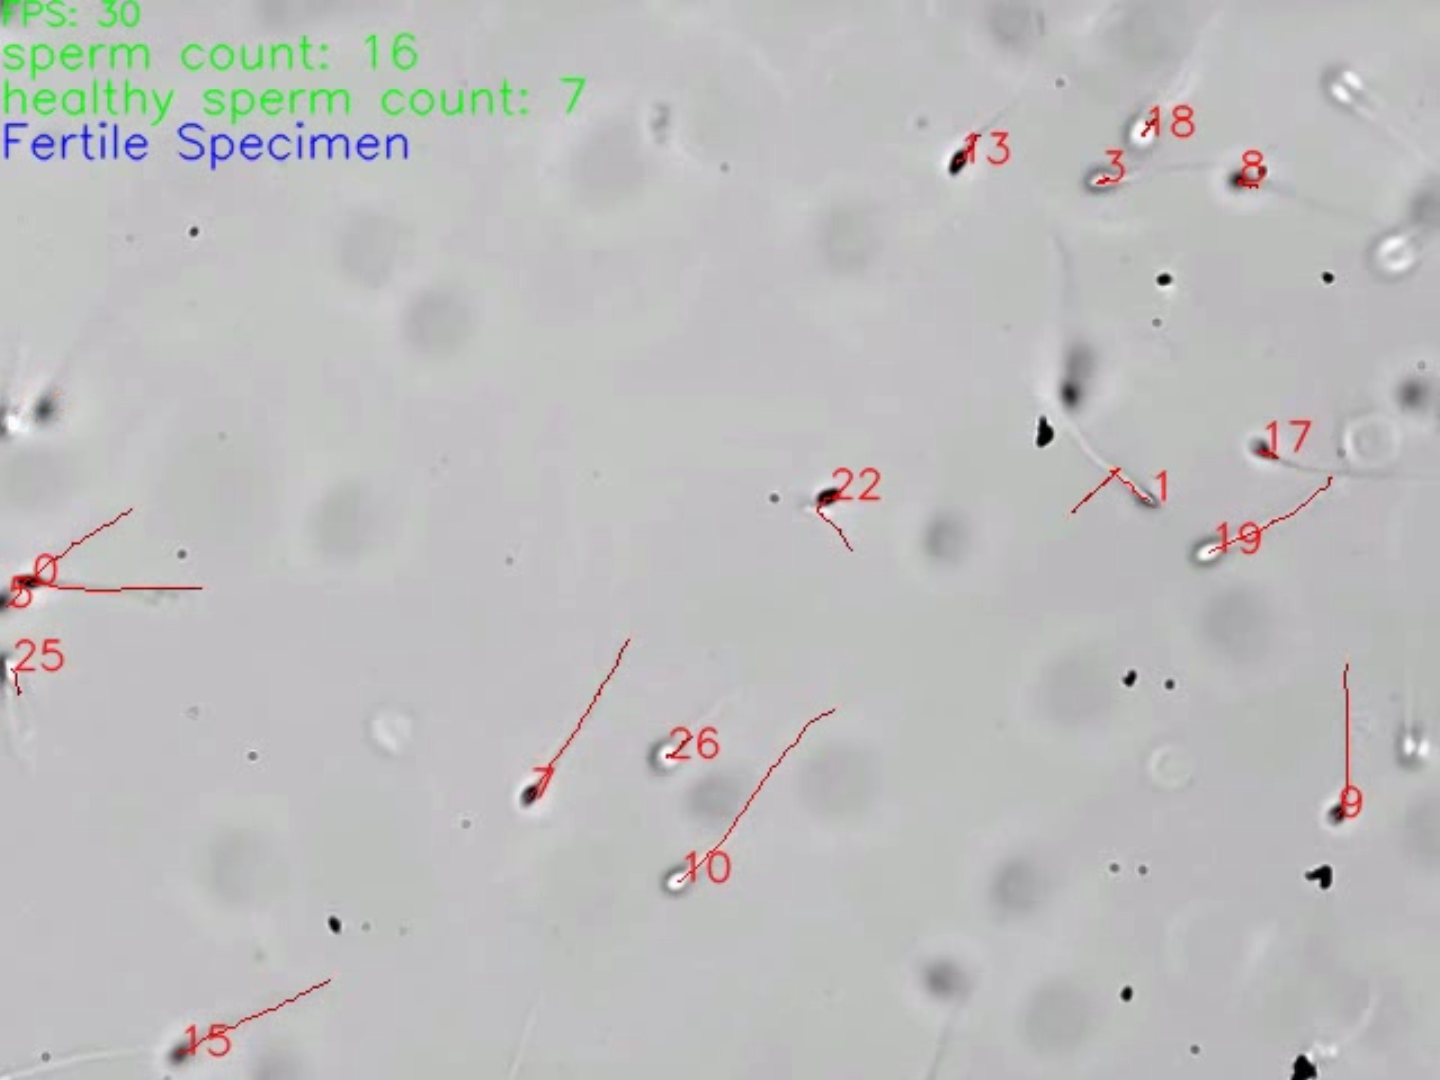
\includegraphics[width=0.75\textwidth]{Images/sam5.png}
    \caption{Sample 5 Output}
    \label{sam5res}
\end{figure}

Even with blurry images, the model still performed quite well. Due to the lower confidence scores, blurry sperms often become undetected from the model and disappear from the video. However, the program keeps track of the sperms even if they are not shown, and the same ID is reassigned to that sperm as soon as the detection is made again. The process can be shown in Figure \ref{sam5keep}.

\begin{figure}[h]
     \centering
     \begin{subfigure}[b]{0.3\textwidth}
         \centering
         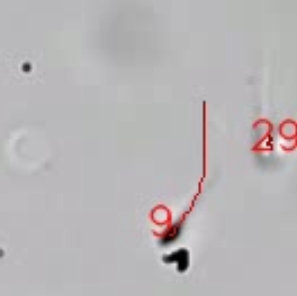
\includegraphics[width=\textwidth]{Images/sam5-4.png}
         \caption{Original Assignment}
     \end{subfigure}
     \hfill
     \begin{subfigure}[b]{0.3\textwidth}
         \centering
         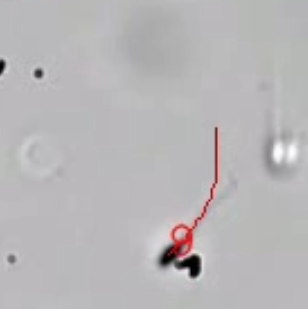
\includegraphics[width=\textwidth]{Images/sam5-5.png}
         \caption{Detection Failure}
     \end{subfigure}
     \hfill
     \begin{subfigure}[b]{0.3\textwidth}
         \centering
         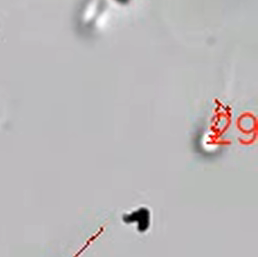
\includegraphics[width=\textwidth]{Images/sam5-6.png}
         \caption{ID Reassigned}
     \end{subfigure}
        \caption{Tracking of Undetected Sperm [ID: 29] in Sample 5}
        \label{sam5keep}
\end{figure}
\newpage
However, there were still a few ID switches, as shown in Figure \ref{sam5switch}.
\begin{figure}[h]
     \centering
     \begin{subfigure}[b]{0.3\textwidth}
         \centering
         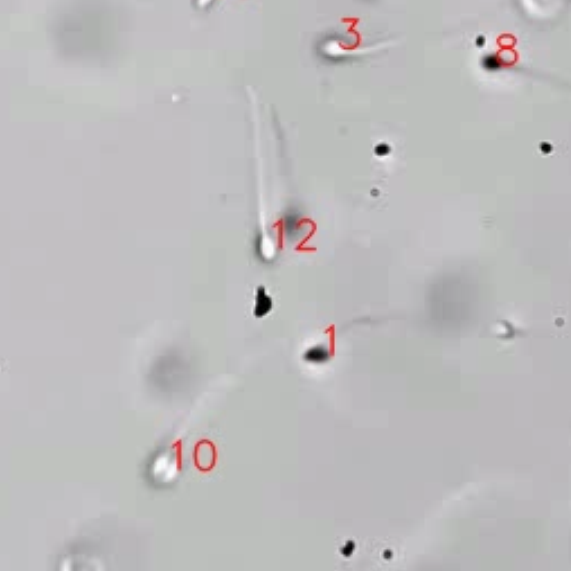
\includegraphics[width=\textwidth]{Images/sam5-1.png}
         \caption{Original Assignment}
     \end{subfigure}
     \hfill
     \begin{subfigure}[b]{0.3\textwidth}
         \centering
         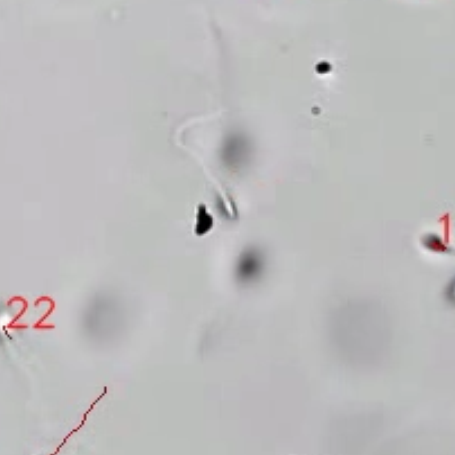
\includegraphics[width=\textwidth]{Images/sam5-2.png}
         \caption{Detection Failure}
     \end{subfigure}
     \hfill
     \begin{subfigure}[b]{0.3\textwidth}
         \centering
         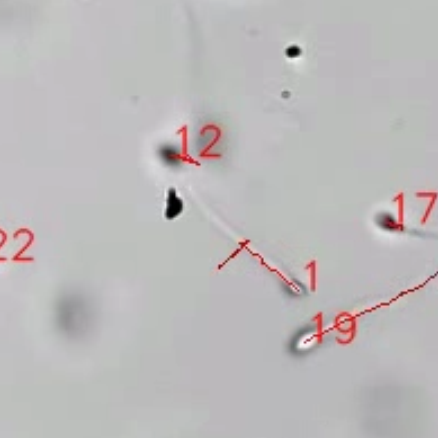
\includegraphics[width=\textwidth]{Images/sam5-3.png}
         \caption{IDs Swapped}
     \end{subfigure}
        \caption{ID Switch [ID: 12, 1] in Sample 5}
        \label{sam5switch}
\end{figure}

This ID switch is due to the short duration of continuous detection of sperm after the initial assignment of ID. The tracking model did not have enough information about the sperms' projected direction. 

This swapping only occurred only once in this sample, and the overall quality of tracking was acceptable. 